%*******************************************************************************
%*********************************** Fifth Chapter *****************************
%*******************************************************************************

\chapter{Density Measurement Induced Dynamics}
% Title of the Fifth Chapter

\ifpdf
    \graphicspath{{Chapter5/Figs/Raster/}{Chapter5/Figs/PDF/}{Chapter5/Figs/}}
\else
    \graphicspath{{Chapter5/Figs/Vector/}{Chapter5/Figs/}}
\fi


\section{Introduction}

In the previous chapter we have introduced a theoretical framework
which will allow us to study measurement backaction using
discontinuous quantum jumps and non-Hermitian evolution due to null
outcomesquantum trajectories. We have also wrapped our quantum gas
model in this formalism by considering ultracold bosons in an optical
lattice coupled to a cavity which collects and enhances light
scattered in one particular direction. One of the most important
conclusions of the previous chapter was that the introduction of
measurement introduces a new energy and time scale into the picture
which competes with the intrinsic dynamics of the bosons.

In this chapter, we investigate the effect of quantum measurement
backaction on the many-body state and dynamics of atoms. In
particular, we will focus on the competition between the backaction
and the the two standard short-range processes, tunnelling and on-site
interactions, in optical lattices. We show that the possibility to
spatially structure the measurement at a microscopic scale comparable
to the lattice period without the need for single site resolution
enables us to engineer efficient competition between the three
processes in order to generate new nontrivial dynamics. However,
unlike tunnelling and on-site interactions our measurement scheme is
global in nature which makes it capable of creating long-range
correlations which enable nonlocal dynamical processes. Furthermore,
global light scattering from multiple lattice sites creates nontrivial
spatially nonlocal coupling to the environment which is impossible to
obtain with local interactions \cite{daley2014, diehl2008,
  syassen2008}. These spatial modes of matter fields can be considered
as designed systems and reservoirs opening the possibility of
controlling dissipations in ultracold atomic systems without resorting
to atom losses and collisions which are difficult to manipulate. Thus
the continuous measurement of the light field introduces a
controllable decoherence channel into the many-body dynamics. Such a
quantum optical approach can broaden the field even further allowing
quantum simulation models unobtainable using classical light and the
design of novel systems beyond condensed matter analogues.

In the weak measurement limit, where the quantum jumps do not occur
frequently compared to the tunnelling rate, this can lead to global
macroscopic oscillations of bosons between odd and even sites. These
oscillations occur coherently across the whole lattice enabled by the
fact that measurement is capable of generating nonlocal spatial
modes. When on-site interactions are included we obtain a system with
three competing energy scales of which two correspond to local
processes and one is global. This complicates the picture
immensely. We show how under certain circumstances interactions
prevent measurement from generating globally coherent dynamics, but on
the other hand when the measurement is strong both processes
collaborate in squeezing the atomic distribution.

On the other end of the spectrum, when measurement is strong we enter
the regime of quantum Zeno dynamics. Frequent measurements can slow
the evolution of a quantum system leading to the quantum Zeno effect
where a quantum state is frozen in its initial configuration
\cite{misra1977, facchi2008}. One can also devise measurements with
multi-dimensional projections which lead to quantum Zeno dynamics
where unitary evolution is uninhibited within this degenerate
subspace, usually called the Zeno subspace \cite{facchi2008,
  raimond2010, raimond2012, signoles2014}. Our flexible setup where global light
scattering can be engineered allows us to suppress or enhance specific
dynamical processes thus realising spatially nonlocal quantum Zeno
dynamics. This unconventional variation occurs when measurement is
near, but not in, its projective limit. The system is still confined
to Zeno subspaces, but intermediate transitions are allowed via
virtual Raman-like processes. We show that this result can, in general
(i.e.~beyond the ultracold gas model), be approximated by a
non-Hermitian Hamiltonian thus extending the notion of quantum Zeno
dynamics into the realm of non-Hermitian quantum mechanics joining the
two paradigms.

\section{Quantum Measurement Induced Dynamics}

\subsection{Large-Scale Dynamics due to Weak Measurement}

We start by considering the weak measurement limit when photon
scattering does not occur frequently compared to the tunnelling rate
of the atoms, i.e.~$\gamma \ll J$. When the system is probed in this
way, the measurement is unable to project the quantum state of the
bosons to an eigenspace as postulated by the Copenhagen interpretation
of quantum mechanics. The backaction of the photodetections is simply
not strong or frequent enough to confine the atoms. However, instead
of confining the evolution of the quantum state, it has been shown in
Refs. \cite{mazzucchi2016, mazzucchi2016njp} that the measurement
leads to coherent global oscillations between the modes generated by
the spatial profile of the light field which we have seen in section
\ref{sec:modes}. Fig. \ref{fig:oscillations} illustrates the atom
number distributions in the odd sites for $Z = 2$ and one of the three
modes for $Z = 3$. These oscillations correspond to atoms flowing from
one mode to another. We only observe a small number of well defined
components which means that this flow happens in phase, all the atoms
are tunnelling between the modes together in unison. Furthermore, this
exchange of population is macroscopic in scale. The trajectories reach
a state where the maximum displacement point corresponds to all the
atoms being entirely within a single mode. Finally, we note that these
oscillating distributions are squeezed by the measurement and the
individual components have a width smaller than the initial state. By
contrast, in the absence of the external influence of measurement
these distributions would spread out significantly and the center of
the broad distribution would oscillate with an amplitude comparable to
the initial imbalance, i.e.~small oscillations for a small initial
imbalance.

\begin{figure}[htbp!]
  \centering
  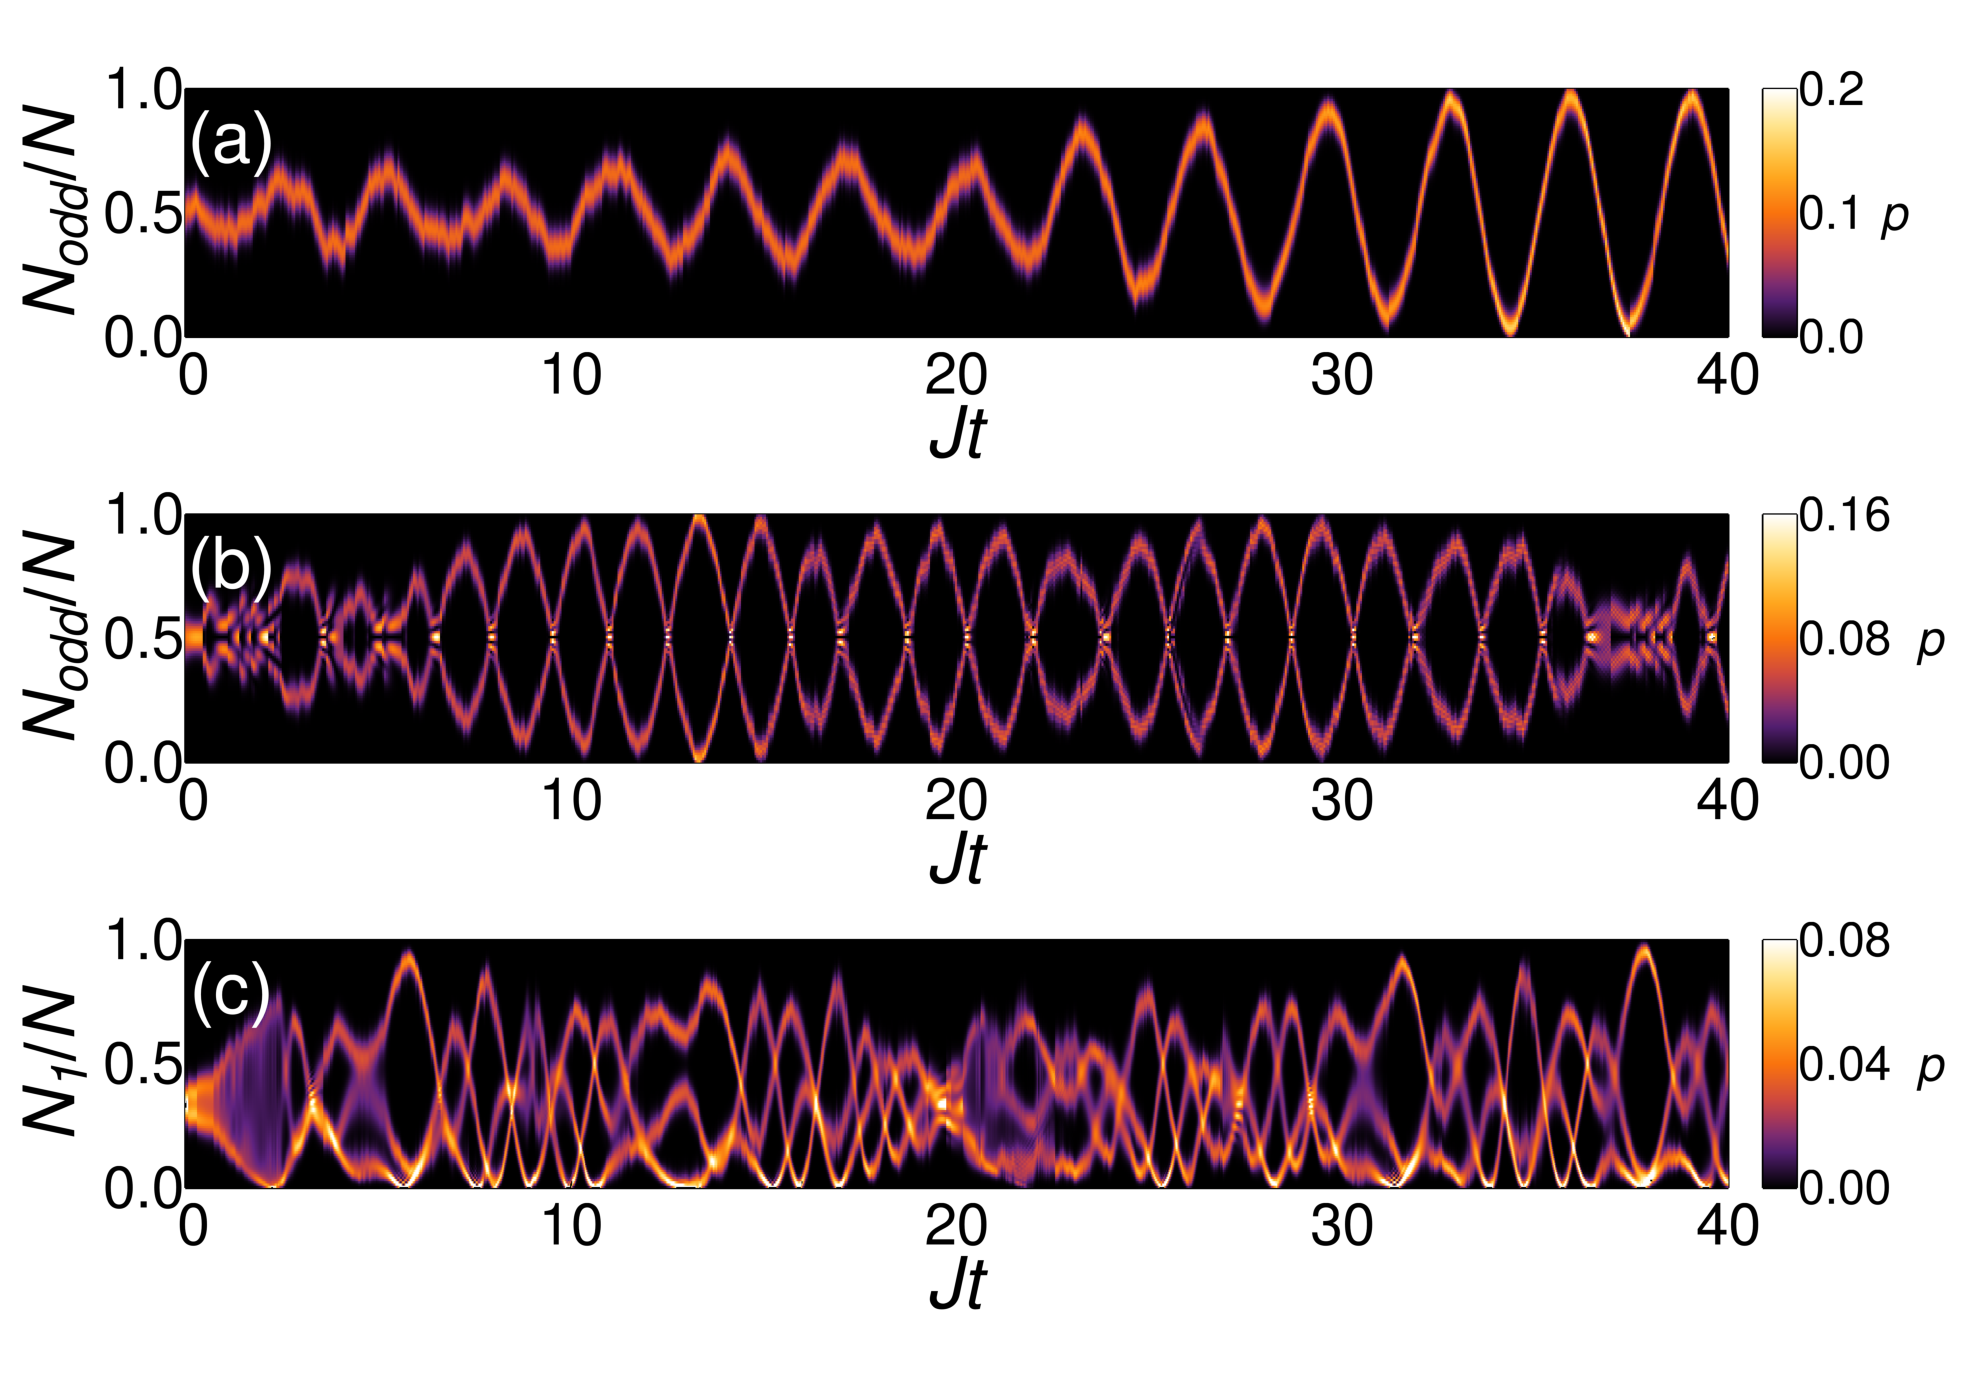
\includegraphics[width=\textwidth]{Oscillations}
  \caption[Macroscopic Oscillations due to Weak Measurement]{Large
    oscillations between the measurement-induced spatial modes
    resulting from the competition between tunnelling and weak
    measurement induced backaction. The plots show the atom number
    distributions $p(N_l)$ in one of the modes in individual quantum
    trajectories. These dstributions show various numbers of
    well-squeezed components reflecting the creation of macroscopic
    superposition states depending on the measurement
    configuration. $U/J = 0$, $\gamma/J = 0.01$, $M=N$, initial
    states: bosonic superfluid. (a) Measurement of the atom number at
    odd sites $\hat{N}_\mathrm{odd}$ creates one strongly oscillating
    component in $p(N_\mathrm{odd})$ ($N = 100$ bosons, $J_{j,j} = 1$
    if $j$ is odd and 0 otherwise). (b) Measurement of
    $(\hat{N}_\mathrm{odd} - \hat{N}_\mathrm{even})^2$ introduces
    $Z = 2$ modes and preserves the superposition of positive and
    negative atom number differences in $p(N_\mathrm{odd})$ ($N = 100$
    bosons, $J_{j,j} = (-1)^{j+1}$). (c) Measurement for $Z = 3$ modes
    preserves three components in $p(N_1)$ ($N = 108$ bosons,
    $J_{j,j} = e^{i 2 \pi j / 3}$).}
  \label{fig:oscillations}
\end{figure}

In Figs. \ref{fig:oscillations}(b,c) we also see that the system is
composed of multiple components. This depends on the quantity that is
being measured and it is a consequence of the fact that the detected
light intensity $\ad_1 \a_1$ is not sensitive to the light phase. The
measurement will not distinguish between permutations of mode
occupations that scatter light with the same intensity, but with a
different phase. For example, when measuring
$\hat{D} = \hat{N}_\mathrm{odd} - \hat{N}_\mathrm{even}$, the light
intensity will be proportional to
$\hat{D}^\dagger \hat{D} = (\hat{N}_\mathrm{odd} -
\hat{N}_\mathrm{even})^2$ and thus it cannot distinguish between a
positive and negative imbalance leading to the two components seen in
Fig. \ref{fig:oscillations}. More generally, the number of components
of the atomic state, i.e.~the degeneracy of $\ad_1 \a_1$, can be
computed from the eigenvalues of Eq. \eqref{eq:Zmodes},
\begin{equation}
  \hat{D} = \sum_l^Z \exp\left[-i 2 \pi l R / Z \right] \hat{N}_l.
\end{equation}
Each eigenvalue can be represented as the sum of the individual terms
in teh above sum which are vectors on the complex plane with phases
that are integer multiples of $2 \pi / Z$: $N_1 e^{-i 2 \pi R / Z}$,
$N_2 e^{-i 4 \pi R / Z}$, ..., $N_Z$. Since the set of possible sums
of these vectors is invariant under rotations by $2 \pi l R / Z$,
$l \in \mathbb{Z}$, and reflection in the real axis, the state of the
system is 2-fold degenerate for $Z = 2$ (reflections leave $Z = 2$
unchanged) and $2Z$-fold degenerate for $Z >
2$. Fig. \ref{fig:oscillations} shows the three mode case, where there
are in fact $6$ components ($2Z = 6$), but in this case they all occur
in pairs resulting in only three visible components.

We will now limit ourselves to a specific illumination pattern with
$\hat{D} = \hat{N}_\mathrm{odd}$ as this leads to the simplest
multimode dynamics with $Z = 2$ and only a single component as seen in
Fig. \ref{fig:oscillations}a, i.e.~no multiple peaks like in
Figs. \ref{fig:oscillations}(b,c). This pattern can be obtained by
crossing two beams such that their projections on the lattice are
identical and the even sites are positioned at their nodes. However,
even though this is the simplest possible case and we are only dealing
with non-interacting atoms solving the full dynamics of the
Bose-Hubbard Hamiltonian combined with measurement is nontrivial. The
backaction introduces a highly nonlinear global term. However, it has
been shown in Ref. \cite{mazzucchi2016njp} that the non-interacting
dynamics with quantum measurement backaction for $Z$-modes reduce to
an effective Bose-Hubbard Hamiltonian with $Z$-sites provided the
initial state is a superfluid. In this simplified model the $N_j$
atoms in the $j$-th site correspond to a superfluid of $N_j$ atoms
within a single spatial mode as defined in section
\ref{sec:modes}. Therefore, we now proceed to study the dynamics for
$\hat{D} = \hat{N}_\mathrm{odd}$ using this reduced effective
double-well model.

The atomic state can be written as
\begin{equation}
  \label{eq:discretepsi}
  | \psi \rangle = \sum_l^N q_l |l, N - l \rangle,
\end{equation}
where the ket $| l, N - l \rangle$, represents a superfluid with $l$
atoms in the odd sites and $N-l$ atoms in the even sites. The
non-Hermitian Hamiltonian describing the time evolution in between the
jumps is given by
\begin{equation}
  \label{eq:doublewell}
  \hat{H} = -J^\mathrm{cl} \left( \bd_o b_e + b_o \bd_e \right) - i
  \gamma \n_o^2
\end{equation}
and the quantum jump operator which is applied at each photodetection
is $\c = \sqrt{2 \kappa} C \n_o$. $b_o$ ($\bd_o$) is the annihilation
(creation) operator in the left site of the effective double-well
corresponding to the superfluid at odd sites of the physical
lattice. $b_e$ ($\bd_e$) is defined similarly, but for the right site
and the superfluid at even sites of the physical lattice.
$\n_o = \bd_o b_o$ is the atom number operator in the left site.

Even though Eq. \eqref{eq:doublewell} is relatively simple as it it is
only a non-interacting two-site model, the non-Hermitian term
complicates the situation making the system difficult to
solve. However, a semiclassical approach to boson dynamics in a
double-well in the limit of many atoms $N \gg 1$ has been developed in
Ref. \cite{juliadiaz2012}. It was originally formulated to treat
squeezing in a weakly interacting bosonic gas, but it can easily be
applied to our system as well. In the limit of large atom number, the
wavefunction in Eq. \eqref{eq:discretepsi} can be described using
continuous variables by defining $\psi (x = l / N) = \sqrt{N}
q_l$. Note that this requires the coefficients $q_l$ to vary smoothly
which is the case for a superfluid state. We now rescale the
Hamiltonian in Eq. \eqref{eq:doublewell} to be dimensionless by
dividing by $NJ^\mathrm{cl}$ and define the relative population
imbalance between the two wells $z = 2x - 1$. Finally, by taking the
expectation value of the Hamiltonian and looking for the stationary
points of
$\langle \psi | \hat{H} | \psi \rangle - E \langle \psi | \psi
\rangle$ we obtain the semiclassical Schr\"{o}dinger equation
\begin{equation}
  \label{eq:semicl}
  i h \partial_t \psi(z, t) = \mathcal{H} \psi(z, t),
\end{equation}
\begin{equation}
  \label{eq:semiH}
  \mathcal{H} \approx -2 h^2 \partial^2_z \psi(z, t) + \left[
    \frac{\omega^2 z^2} {8} - \frac{i \Gamma} {4} \left( z + 1
    \right)^2 \right] \psi(z, t),
\end{equation}
where $\Gamma = N \kappa |C|^2 / J$, $h = 1/N$,
$\omega = 2 \sqrt{1 + \Lambda - h}$, and
$\Lambda = NU / (2J^\mathrm{cl})$. The full derivation is not
straightforward, but the introduction of the non-Hermitian term
requires only a minor modification to the original formalism presented
in detail in Ref. \cite{juliadiaz2012} so we have omitted it here. We
will also be considering $U = 0$ as the effective model is only valid
in this limit, thus $\Lambda = 0$. However, this model is valid for an
actual physical double-well setup in which case interacting bosons can
also be considered. The equation is defined on the interval
$z \in [-1, 1]$, but $z \ll 1$ has been assumed in order to simplify
the kinetic term and approximate the potential as parabolic. This does
mean that this approximation is not valid for the maximum amplitude
oscillations seen in Fig. \ref{fig:oscillations}a, but since they
already appear early on in the trajectory we are able to obtain a
valid analytic description of the oscillations and their growth.

A superfluid state in our continuous variable approximation
corresponds to a Gaussian wavefunction $\psi$. Furthermore, since the
potential is parabolic, even with the inclusion of the non-Hermitian
term, it will remain Gaussian during subsequent time
evolution. Therefore, we will use a very general Gaussian wavefunction
of the form
\begin{equation}
  \label{eq:ansatz}
  \psi(z, t) = \frac{1}{\pi b^2}\exp\left[ i \epsilon 
  - \frac{(z - z_0)^2} {2 b^2} + \frac{i \phi (z - z_\phi)^2} {2 b^2} \right]
\end{equation}
as our ansatz to Eq. \eqref{eq:semicl}. The parameters $b$, $\phi$,
$z_0$, and $z_\phi$ are real-valued functions of time whereas
$\epsilon$ is a complex-valued function of time. Physically, the value
$b^2$ denotes the width, $z_0$ the position of the center, $\phi$ and
$z_\phi$ contain the local phase information, and $\epsilon$ only
affects the global phase and norm of the Gaussian wave packet.

The non-Hermitian Hamiltonian and an ansatz are not enough to describe
the full dynamics due to measurement. We also need to know the effect
of each quantum jump. Within the continuous variable approximation,
our quantum jump become $\c \propto 1 + z$. We neglect the constant
prefactors, because the wavefunction is normalised after a quantum
jump. Expanding around the peak of the Gaussian ansatz we get
\begin{equation}
  1 + z \approx \exp \left[ \ln (1 + z_0) + \frac{z - z_0}{1 + z_0} -
    \frac{(z - z_0)^2}{2 (1 + z_0)^2} \right].
\end{equation}
Multiplying the wavefunction in Eq. \eqref{eq:ansatz} with the jump
operator above yields a Gaussian wavefunction as well, but the
parameters change discontinuously according to
\begin{align}
  \label{eq:jumpb2}
  b^2 & \rightarrow \frac{ b^2 (1 + z_0)^2 } { (1 + z_0)^2 + b^2 }, \\
  \phi & \rightarrow \frac{ \phi (1 + z_0)^2 } { (1 + z_0)^2 + b^2 }, \\
  \label{eq:jumpz0}
  z_0 & \rightarrow z_0 + \frac{ b^2 (1 + z_0) } { (1 + z_0)^2 + b^2}, \\
  z_\phi & \rightarrow z_\phi, \\
  \epsilon & \rightarrow \epsilon.
\end{align}
The fact that the wavefunction remains Gaussian after a photodetection
is a huge advantage, because it means that the combined time evolution
of the system can be described with a single Gaussian ansatz in
Eq. \eqref{eq:ansatz} subject to non-Hermitian time evolution
according to Eq. \eqref{eq:semicl} with discontinous changes to the
parameter values at each quantum jump.

Having identified an appropriate ansatz and the effect of quantum
jumps we proceed with solving the dynamics of wavefunction in between
the photodetecions. The initial values of the parameters for a
superfluid state of $N$ atoms across the whole lattice are $b^2 = 2h$,
$\phi =0$, $a_0 = 0$, $a_\phi = 0$, $\epsilon = 0$. However, we use
the most general initial conditions at time $t = t_0$ which we denote
by $b(t_0) = b_0$, $\phi(t_0) = \phi_0$, $z_0(t_0) = a_0$,
$z_\phi(t_0) = a_\phi$, and $\epsilon(t_0) = \epsilon_0$. The reason
for keeping them as general as possible is that after every quantum
jump the system changes discontinuously. The subsequent time evolution
is obtained by solving the Schr\"{o}dinger equation with the post-jump
paramater values as the new initial conditions.

By plugging the ansatz in Eq. \eqref{eq:ansatz} into the
Schr\"{o}dinger equation in Eq. \eqref{eq:semicl} we obtain three
differential equations
\begin{equation}
  \label{eq:p}
  -2 h^2 p^2 + \left( \frac{ \omega^2 } { 8 } - \frac{ i \Gamma } { 4
    } \right) + \frac{ i h } { 2 } \frac{ \mathrm{d} p } { \mathrm{d}
    t } = 0,
\end{equation}
\begin{equation}
  \label{eq:pq}
  4 h^2 p q - \frac{ i \Gamma } { 2 } - i h \frac{ \mathrm{d} q } {
    \mathrm{d} t } = 0
\end{equation}
\begin{equation}
  \label{eq:pqr}
  -2 h^2 (q^2 - p) - \frac{ i \Gamma } { 4 } - i h \left( \frac{ 1 } {
      4 x } \frac{ \mathrm{d} x } {\mathrm{d} t } + i \frac{
      \mathrm{d} \epsilon } { \mathrm{d} t } - \frac{1}{2} \frac{
      \mathrm{d} r } { \mathrm{d} t } \right) = 0,
\end{equation}
where $x = 1/b^2$, $p = (1 - i \phi)/b^2$,
$q = (z_0 - i \phi z_\phi)/b^2$, and
$r = (z_0^2 - \phi z_\phi^2)/b^2$. The corresponding initial
conditions are $x(t_0) = x_0 = 1/b_0^2$,
$p(t_0) = p_0 = (1 - i \phi_0)/b_0^2$,
$q(t_0) = q_0 = (a_0 - \phi_0 a_\phi)/b_0^2$, and
$r(t_0) = r_0 = (a_0^2 - \phi_0 a_\phi^2)/b_0^2$. The original
parameters can be extracted from these auxiliary variables by
$b^2 = 1 / \Re \{ p \}$, $\phi = - \Im \{ p \} / \Re \{ p \}$,
$z_0 = \Re \{ q \} / \Re \{ p \}$,
$z_\phi = \Im \{ q \} / \Im \{ p \}$, and $\epsilon$ appears
explicitly in the equations above.

First, it is worth noting that all parameters of interest can be
extracted from $p(t)$ and $q(t)$ alone. We are not interested in
$\epsilon$ as it is only related to the global phase and the norm of
the wavefunction and it contains little physical
information. Furthermore, an interesting and incredibly convenient
feature of these equations is that the Eq. \eqref{eq:p} is a function
of $p(t)$ alone and Eq. \eqref{eq:pq} is a function of $p(t)$ and
$q(t)$ only. Therefore, we only need to solve first two equations and
we can neglect Eq. \eqref{eq:pqr}. However, in order to actually
perform Monte-Carlo simulations of quantum trajectories
Eq. \eqref{eq:pqr} would need to be solved in order to obtain correct
jump statistics.

We start with Eq. \eqref{eq:p} and we note it can be rearranged into
the form
\begin{equation}
  \frac{ \mathrm{d} p } { (\zeta \omega / 4 h)^2 - p^2 } = i 4 h
  \mathrm{d} t,
\end{equation}
where $\zeta^2 = (\alpha - i \beta)^2 = 1 - i 2 \Gamma / \omega^2$, and
\begin{equation}
  \alpha = \sqrt{ \frac{1}{2} + \frac{1}{2} \sqrt{1 + \frac{ 4\Gamma^2
      }{ \omega^4 }}},
\end{equation}
\begin{equation}
  \beta = -\sqrt{ -\frac{1}{2} + \frac{1}{2} \sqrt{1 + \frac{ 4\Gamma^2
      }{ \omega^4 }}}.
\end{equation}
This is a standard integral\footnotemark and thus yields
\begin{equation}
  \label{eq:psol}
  p(t) = \frac{ \zeta \omega } { 4 h } 
  \frac{ ( \zeta \omega + 4 h p_0 )e^{i \zeta \omega t} - ( \zeta
    \omega - 4 h p_0 ) e^{-i \zeta \omega t} }
  { ( \zeta \omega + 4 h p_0 )e^{i \zeta \omega t} + ( \zeta \omega
    - 4 h p_0 ) e^{-i \zeta \omega t} }.
\end{equation}

\footnotetext{ \[ \int \frac{\mathrm{d} x}{a^2 - x^2} = \frac{1}{2a}
    \ln \left( \frac{a+x}{a-x} \right) + \mathrm{const.} 
    \quad\quad\quad\quad\quad\quad\quad\quad\quad\quad\quad\quad\quad\quad\quad
    \quad\quad\quad\quad\quad\] }

Having found an expression for $p(t)$ we can now solve
Eq. \eqref{eq:pq} for $q(t)$. To do that we first define the
integrating factor
\begin{equation}
  I(t) = \exp \left[ i 4 h \int p \mathrm{d} t \right] = ( \zeta
  \omega + 4 h p_0 )e^{i \zeta \omega t} + ( \zeta \omega - 4 h p_0 )
  e^{-i \zeta \omega t},
\end{equation}
which lets us rewrite Eq. \eqref{eq:pq} as
\begin{equation}
  \label{eq:Iq}
  \frac{\mathrm{d}} {\mathrm{d} t}(Iq) = - \frac{\Gamma}{2 h} I.
\end{equation}
%Upon integrating the equation above we obtain
%\begin{equation}
%  \label{eq:Iq}
%  Iq = - \frac{ \Gamma } {2 h} \int I \mathrm{d} t.
%\end{equation}
Upon integrating and the substitution of the explicit form of the
integration factor into this equation we obtain the solution
\begin{equation}
  \label{eq:qsol}
  q(t) = \frac{1}{2 h \zeta \omega} 
  \frac{4 h \zeta^2 \omega^2 q_0 - i 8 h \Gamma p_0
    + i \Gamma [( \zeta \omega + 4 h p_0 )e^{i \zeta \omega t} - 
    ( \zeta \omega - 4 h p_0 )e^{-i \zeta \omega t}]}
  { ( \zeta \omega + 4 h p_0 )e^{i \zeta \omega t} + 
    ( \zeta \omega - 4 h p_0 )e^{-i \zeta \omega t}}.
\end{equation}

The solutions we have obtained to $p(t)$ in Eq. \eqref{eq:psol} and
$q(t)$ in Eq. \eqref{eq:qsol} are sufficient to completely describe
the physics of the system. Unfortunately, these expressions are fairly
complex and it is difficult to extract the physically meaningful
parameters in a form that is easy to analyse. Therefore, we instead
consider the case when $\Gamma = 0$, but we do not neglect the effect
of quantum jumps. It may seem counter-intuitive to neglect the term
that appears due to measurement, but we are considering the weak
measurement regime where $\gamma \ll J^\mathrm{cl}$ and thus the
dynamics between the quantum jumps are actually dominated by the
tunnelling of atoms rather than the null outcomes. Furthermore, the
effect of the quantum jump is independent of the value of $\Gamma$
($\Gamma$ only determined their frequency). However, this is only true
at times shorter than the average time between two consecutive quantum
jumps. Therefore, this approach will not yield valid answers on the
time scale of a whole quantum trajectory, but it will give good
insight into the dynamics immediately after a quantum jump. The
solutions for $\Gamma = 0$ are
\begin{equation}
b^2(t) = \frac{b_0^2}{2} \left[ \left(1 + \frac{16 h^2 (1 + \phi_0^2)}
    {b_0^4 \omega^2} \right) + \left(1 - \frac{16 h^2 (1 + \phi_0^2)}
    {b_0^4 \omega^2} \right) \cos (2 \omega t) + \frac{8 h \phi_0}{b_0^2
    \omega} \sin(2 \omega t) \right],
\end{equation}
\begin{equation}
  \phi(t) = \frac{b_0^2 \omega} {8 h} \left[ \left( \frac{16 h^2 (1 + \phi_0^2)}
      {b_0^4 \omega^2} - 1 \right) \sin (2 \omega t) + \frac{8 h
      \phi_0} {b_0^2 \omega} \cos (2 \omega t) \right],
\end{equation}
\begin{equation}
  z_0(t) = a_0 \cos(\omega t) + \frac{4 h \phi_0} {b_0^2 \omega} (a_0 -
  a_\phi) \sin (\omega t),
\end{equation}
\begin{equation}
  \phi(t) z_\phi(t) = \phi_0 a_\phi \cos (\omega t)  + \frac{4 h}
  {b_0^2 \omega} (a_0 - \phi_0^2 a_\phi) \sin( \omega t).
\end{equation}
First, these equations show that all quantities oscillate with a
frequency $\omega$ or $2 \omega$. We are in particular interested in
the quantity $z_0(t)$ as it represents the position of the peak of the
wavefunction and we see that it oscillates with an amplitude
$\sqrt{a_0^2 + 16 h^2 \phi_0^2 (a_0 - a_\phi)^2 / (b_0^4
  \omega^2)}$. Thus we have obtained a solution that clearly shows
oscillations of a single Gaussian wave packet. The fact that this
appears even when $\Gamma = 0$ shows that the oscillations are a
property of the Bose-Hubbard model itself. However, they also depend
on the initial conditions and for these oscillations to occur, $a_0$
and $a_\phi$ cannot be zero, but this is exactly the case for an
initial superfluid state. We have seen in Eq. \eqref{eq:jumpz0} that
the effect of a photodetection is to displace the wavepacket by
approximately $b^2$, i.e.~the width of the Gaussian, in the direction
of the positive $z$-axis. Therefore, even though the can oscillate in
the absence of measurement it is the quantum jumps that are the
driving force behind this phenomenon. Furthermore, these oscillations
grow because the quantum jumps occur at an average instantaneous rate
proportional to $\langle \cd \c \rangle (t)$ which itself is
proportional to $(1+z)^2$. This means they are most likely to occur at
the point of maximum displacement in the positive $z$ direction at
which point a quantum jump provides positive feedback and further
increases the amplitude of the wavefunction leading to the growth seen
in Fig. \ref{fig:oscillations}a. The oscillations themselves are
essentially due to the natural dynamics of coherently displaced atoms
in a lattice , but it is the measurement that causes the initial and
more importantly coherent displacement and the positive feedback drive
which causes the oscillations to continuously grow.

We have now seen the effect of the quantum jumps and how that leads to
oscillations between odd and even sites in a lattice. However, we have
neglected the effect of null outcomes on the dynamics. Even though it
is small, it will not be negligible on the time scale of a quantum
trajectory with multiple jumps. First, we note that all the
oscillatory terms $p(t)$ and $q(t)$ actually appear as
$\zeta \omega = (\alpha - i \beta) \omega$. Therefore, we can see that
the null outcomes lead to two effects: an increase in the oscillation
frequency by a factor of $\alpha$ to $\alpha \omega$ and a damping
term with a time scale $1/(\beta \omega)$. For weak measurement, both
$\alpha$ and $\beta$ will be close to $1$ so the effects are not
visible on short time scales. Instead, we look at the long time
limit. Unfortunately, since all the quantities are oscillatory a
stationary long time limit does not exist especially since the quantum
jumps provide a driving force. However, the width of the Gaussian,
$b^2$, is unique in that it doesn't oscillate around $b^2 =
0$. Furthermore, from Eq. \eqref{eq:jumpb2} we see that even though it
will decrease discontinuously at every jump, this effect is fairly
small since $b^2 \ll 1$ generally. Therefore, we expect $b^2$ to
oscillate, but with an amplitude that decreases approximately
monotonically with time due to quantum jumps and the
$1/(\beta \omega)$ decay terms, because unlike for $z_0$ the quantum
jumps do not cause further displacement in this quantity. Thus,
neglecting the effect of quantum jumps and taking the long time limit
yields
\begin{equation}
  \label{eq:b2}
  b^2(t \rightarrow \infty) = \frac{4 h} {\gamma \omega} \approx
  b^2_\mathrm{SF} \left( 1 - \frac{\Gamma^2}{32} \right),
\end{equation}
where the approximation on the right-hand side follows from the fact
that $\omega \approx 2$ since we are considering the $N \gg 1$ limit,
and because we are considering the weak measurement limit
$\Gamma^2 / \omega^4 \ll 1$. $b^2_\mathrm{SF} = 2h$ denotes the width
of the initial superfluid state. This result is interesting, because
it shows that the width of the Gaussian distribution is squeezed as
compared with its initial state which is exactly what we see in
Fig. \ref{fig:oscillations}a. However, if we substitute the parameter
values used in that trajectory we only get a reduction in width by
about $3\%$, but the maximum amplitude oscillations in look like they
have a significantly smaller width than the initial distribution. This
discrepancy is due to the fact that the continuous variable
approximation is only valid for $z \ll 1$ and thus it cannot explain
the final behaviour of the system. Furthermore, it has been shown that
the width of the distribution $b^2$ does not actually shrink to a
constant value, but rather it keeps oscillating around the value given
in Eq. \eqref{eq:b2} \cite{mazzucchi2016njp}. However, what we do see
is that during the early stages of the trajectory, which are well
described by this model, is that the width does in fact stay roughly
constant. It is only in the later stages when the oscillations reach
maximal amplitude that the width becomes visibly reduced.

\subsection{Three-Way Competition}

Now it is time to turn on the inter-atomic interactions,
$U/J^\mathrm{cl} \ne 0$. As a result the atomic dynamics will change
as the measurement now competes with both the tunnelling and the
on-site interactions. A common approach to study such open systems is
to map a dissipative phase diagram by finding the steady state of the
master equation for a range of parameter values
\cite{kessler2012}. However, here we adopt a quantum optical approach
in which we focus on the conditional dynamics of a single quantum
trajectory as this corresponds to a single realisation of an
experiment. The resulting evolution does not necessarily reach a
steady state and usually occurs far from the ground state of the
system.

A key feature of the quantum trajectory approach is that each
trajectory evolves differently as it is conditioned on the
photodetection times which are determined stochastically. Furthermore,
even states in the same measurement subspace, i.e.~indistinguishable
to the measurement , can have minimal overlap. This is in contrast to
the unconditioned solutions obtained with the master equation which
only yields a single outcome that is an average taken over all
possible outcomes. However, this makes it difficult to study the
three-way competition in some meaningful way across the whole
parameter range.

Ultimately, regardless of its strength measurement always tries to
project the quantum state onto one of its eigenstates (or eigenspaces
if there are degeneracies). If the probe is strong enough this will
succeed, but we have seen in the previous section that when this is
not the case, measurement leads to new dynamical phenomena. However,
despite this vast difference in behaviour, there is a single quantity
that lets us determine the degree of success of the projection, namely
the fluctuations, $\sigma_D^2$ (or equivalently the standard
deviation, $\sigma_D$), of the observable that is being measured,
$\hat{D}$. For a perfect projection this value is exactly zero,
because the system at that point is in the corresponding
eigenstate. When the system is unable to project the state into such a
state, the variance will be non-zero. However, the smaller its value
is the closer it is to being in such an eigenstate and on the other
hand a large variance means that the internal processes dominate the
competition. Finally, this quantity is perfect to study quantum
trajectories, because its value in the long-time limit it is only a
function of $\gamma$, $J$, and $U$. It does not depend on the explicit
history of photodetections. Fig. \ref{fig:squeezing} shows a plot of
this quantity for $\hat{D} = \hat{N}_\mathrm{odd}$ averaged over
multiple trajectories, $\langle \sigma^2_D \rangle_\mathrm{traj}$, as
a function of $\gamma/J$ and $U/J$ for a lattice of six atoms on six
sites (we cannot use the effective double-well model, because
$U \ne 0$). We use a ground state of for the corresponding $U$ and $J$
values as this provides a realistic starting point and a reference for
comparing the measurement induced dynamics. We will also consider only
$\hat{D} = \hat{N}_\mathrm{odd}$ unless stated otherwise.

\begin{figure}[htbp!]
  \centering
  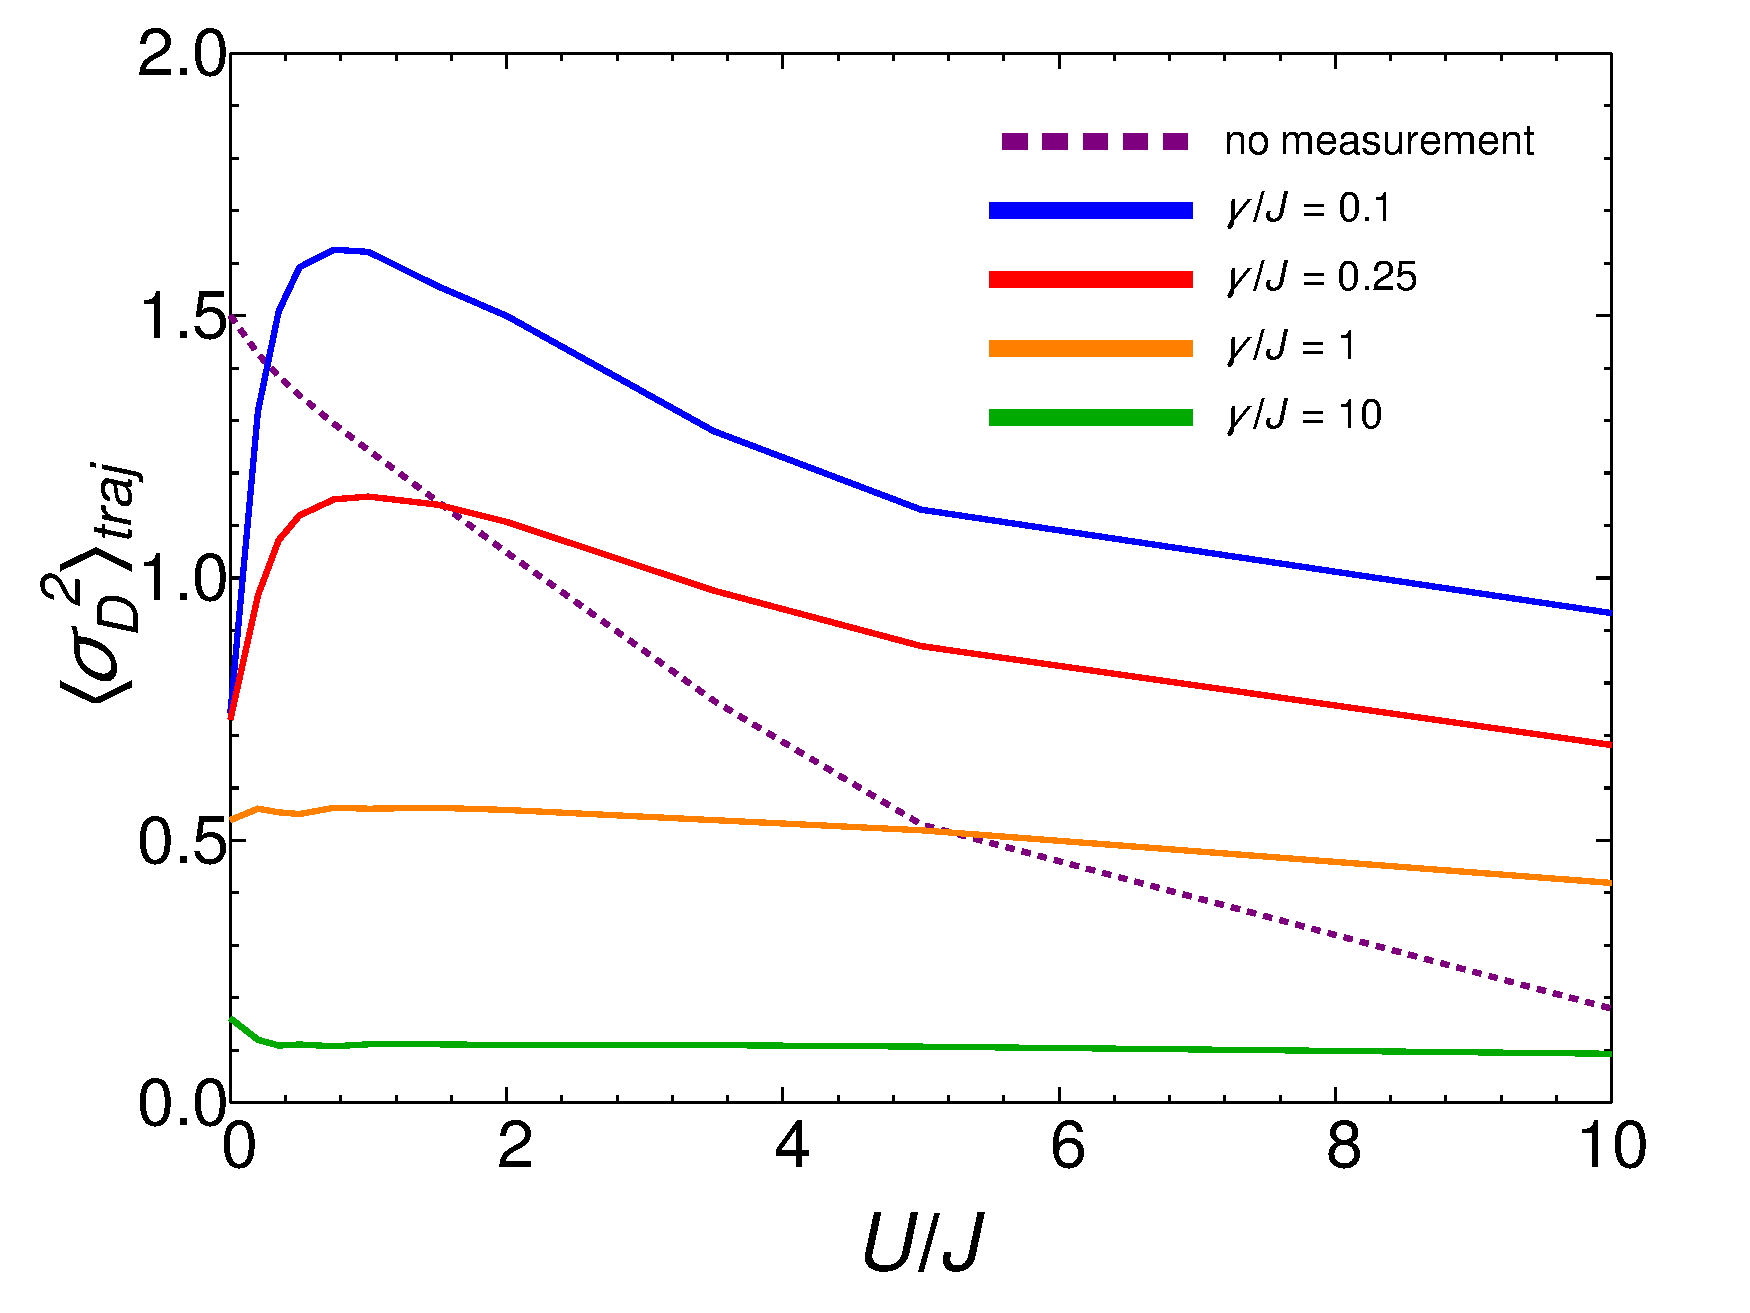
\includegraphics[width=\textwidth]{Squeezing}
  \caption[Squeezing in the presence of Interactions]{Atom number
    fluctuations at odd sites for for $N = 6$ atoms at $M = 6$ sites
    subject to a $\hat{D} = \hat{N}_\mathrm{odd}$ measurement
    demonstrating the competition of global measurement with local
    interactions and tunnelling. Number variances are averaged over
    100 trajectories. Error bars are too small to be shown
    ($\sim 1\%$) which emphasizes the universal nature of the
    squeezing. The initial state used was the ground state for the
    corresponding $U$ and $J$ value. The fluctuations in the ground
    state without measurement decrease as $U / J$ increases,
    reflecting the transition between the supefluid and Mott insulator
    phases. For weak measurement values
    $\langle \sigma^2_D \rangle_\mathrm{traj}$ is squeezed below the
    ground state value for $U = 0$, but it subsequently increases and
    reaches its maximum as the atom repulsion prevents the
    accumulation of atoms prohibiting coherent oscillations thus
    making the squeezing less effective. In the strongly interacting
    limit, the Mott insulator state is destroyed and the fluctuations
    are larger than in the ground state as weak measurement isn't
    strong enough to project into a state with smaller fluctuations
    than the ground state.}
  \label{fig:squeezing}
\end{figure}

First, it is important to note that even though we are dealing with an
average over many trajectories this information cannot be extracted
from a master equation solution. This is because the variance of
$\hat{D}$ as calculated from the density matrix would be dominated by
the uncertainty of the final state. In other words, the fact that the
final value of $\hat{D}$ is undetermined is included in this average
and thus the fluctuations obtained this way are representative of the
variance in the final outcome rather than the squeezing of an
individual conditioned trajectory. This highlights the fact that
interesting physics happens on a single trajectory level which would
be lost if we studied an ensemble average.

\begin{figure}[htbp!]
  \centering
  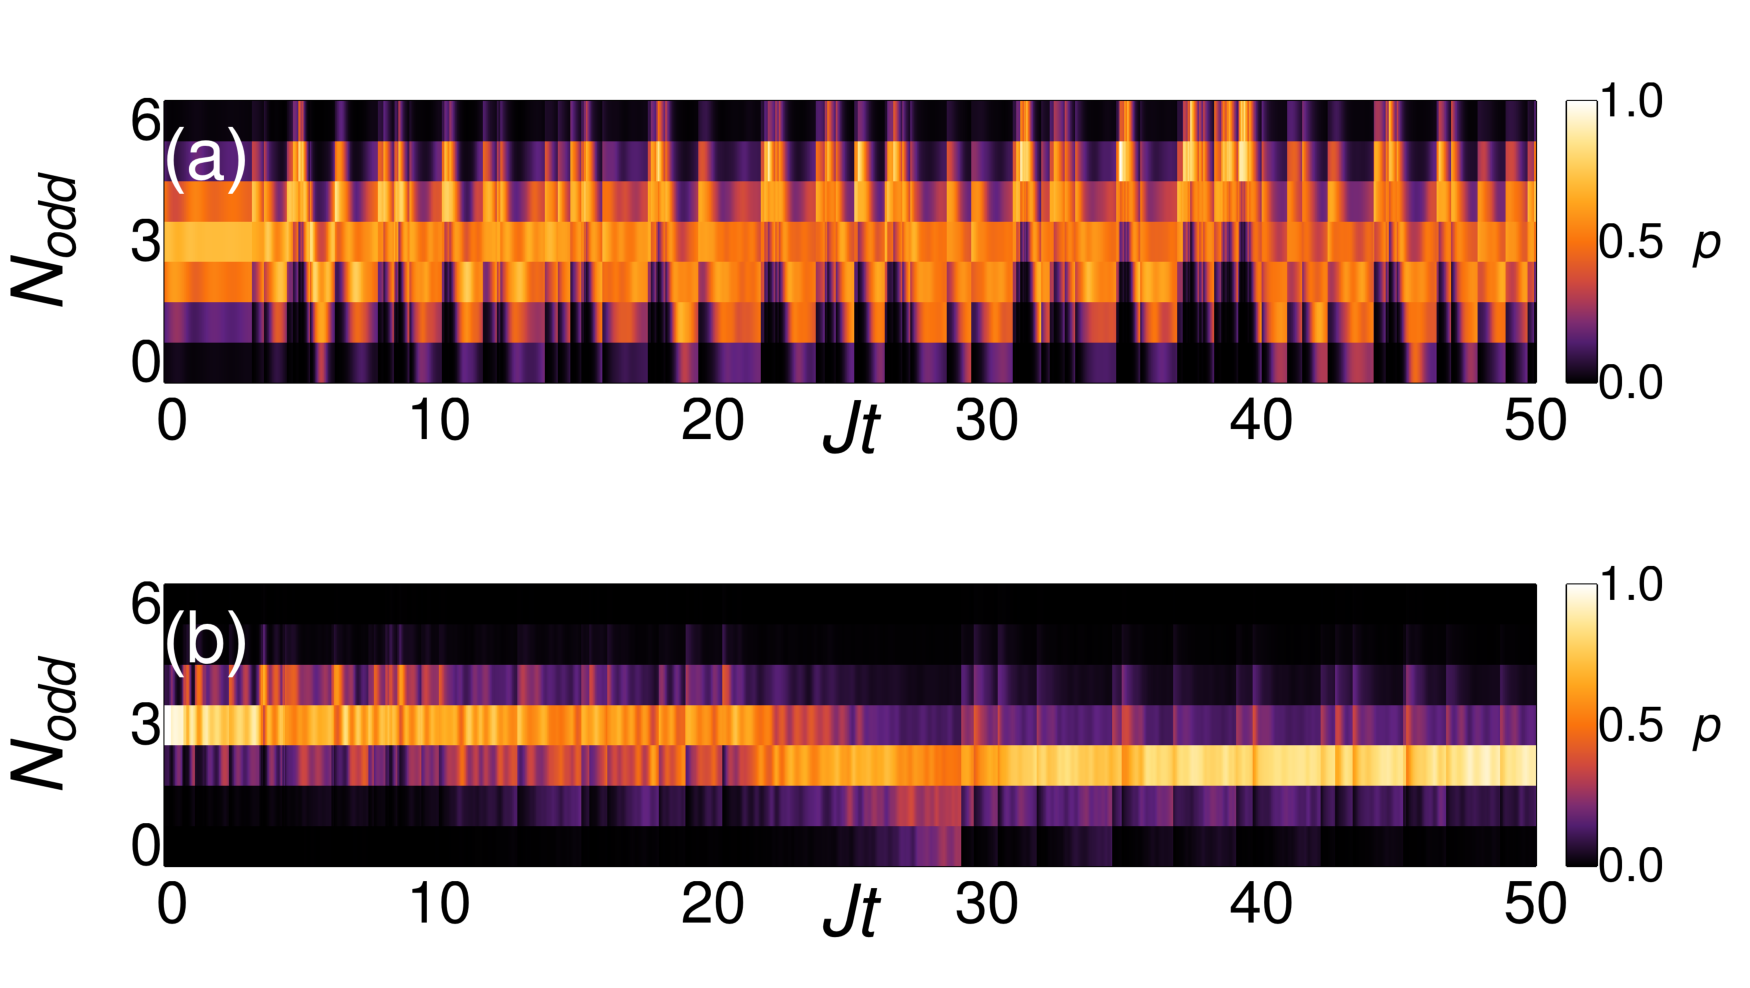
\includegraphics[width=\textwidth]{panel_U}
  \caption[Trajectories in the presence of Interactions]{Conditional
    dynamics of the atom-number distributions at odd sites
    illustrating competition of the global measurement with local
    interactions and tunnelling. The plots are for single quantum
    trajectores starting from the ground state for $N = 6$ atoms on
    $M = 6$ sites with $\hat{D} = \hat{N}_\mathrm{odd}$,
    $\gamma/J = 0.1$. (a) Weakly interacting bosons $U/J = 1$: the
    on-site repulsion prevents the formation of well-defined
    oscillation in the population of the mode. As states with
    different imbalance evolve with different frequencies, the
    squeezing is not as efficient for the non-interacting case. (b)
    Strongly interacting bosons $U/J = 10$: oscillations are
    completely supressed and the number of atoms in the mode is rather
    well-defined although clearly worse than in a Mott insulator.}
  \label{fig:Utraj}
\end{figure}

Looking at Fig. \ref{fig:squeezing} we see many interesting things
happening suggesting different regimes of behaviour. For the ground
state (i.e.~no measurement) we see that the fluctuations decrease
monotonically as $U$ increases reflecting the superfluid to Mott
insulator quantum phase transition. The measured state on the other
hand behaves very differently and
$\langle \sigma^2_D \rangle_\mathrm{traj}$ varies
non-monotonically. For weak interactions the fluctuations are strongly
squeezed below those of the ground state followed by a rapid increase
as $U$ is increased before peaking and eventually decreasing. We have
already seen in the previous section and in particular
Fig. \ref{fig:oscillations} that the macroscopic oscillations at
$U = 0$ are well squeezed when compared to the inital state and this
is the case over here as well. However, as $U$ is increased the
interactions prevent the atoms from accumulating in one place thus
preventing oscillations with a large amplitude which effectively makes
the squeezing less effective as seen in Fig. \ref{fig:Utraj}a. In
fact, we have seen towards the end of the last section how for small
amplitude oscillations that can be described by the effective
double-well model the width of the number distribution does not change
by much. Even though that model is not valid for $U \ne 0$ we should
not be surprised that without macroscopic oscillations the
fluctuations cannot be significantly reduced.

On the other end of the spectrum, for weak measurement, but strong
on-site interactions we note that the backaction leads to a
significant increase in fluctuations compared to the ground
state. This is simply due to the fact that the measurement destroys
the Mott insulating state, which has small fluctuations due to strong
local interactions, but then subsequently is not strong enough to
squeeze the resulting dynamics as shown in Fig. \ref{fig:Utraj}b. To
see why this is so easy for the quantum jumps to do we look at the
ground state in first-order perturbation theory given by
\begin{equation}
  | \Psi_{J/U} \rangle = \left[ 1 + \frac{J}{U} \sum_{\langle i, j
      \rangle} \bd_i b_j \right] | \Psi_0 \rangle,
\end{equation}
where we have neglected the non-Hermitian term as we're in the weak
measurement regime and $| \Psi_0 \rangle$ is the Mott insulator state and the second
term in the brackets represents a uniform distribution of
particle-hole excitation pairs across the lattice. In the
$U \rightarrow \infty$ limit a quantum jump has no effect as
$| \Psi_0 \rangle$ is already an eigenstate of $\hat{D}$. However, for
finite $U$, each photocount will amplify the present excitations
increasing the fluctuations in the system. In fact, consecutive
detections lead to an exponential growth of these excitations. For
$K \gg 1$ illuminated sites and unit filling of the lattice, the
atomic state after $m$ consecutive quantum jumps becomes
$\c^m | \Psi_{J/U} \rangle \propto | \Psi_{J/U} \rangle + | \Phi_m
\rangle$ where
\begin{equation}
  | \Phi_m \rangle = \frac{2^m J} {K U} \sum_{i \in
    \mathrm{odd}} \left( \bd_i b_{i-1} - \bd_{i-1} b_i - \bd_{i+1} b_i
    + \bd_i b_{i+1} \right) | \Psi_0 \rangle.
\end{equation}
In the weak measurement regime the effect of non-Hermitian decay is
negligible compared to the local atomic dynamics combined with the
quantum jumps so there is minimal dissipation occuring. Therefore,
because of the exponential growth of the excitations, even a small
number of photons arriving in succession can destroy the ground
state. We have neglected all dynamics in between the jumps which would
distribute the new excitations in a way which will affect and possibly
reduce the effects of the subsequent quantum jumps. However, due to
the lack of any decay channels they will remain in the system and
subsequent jumps will still amplify them further destroying the ground
state and thus quickly leading to a state with large fluctuations.

In the strong measurement regime ($\gamma \gg J$) the measurement
becomes more significant than the local dynamics and the system will
freeze the state in the measurement operator eigenstates. In this
case, the squeezing will always be better than in the ground state,
because measurement and on-site interaction cooperate in suppressing
fluctuations. This cooperation did not exist for weak measurement,
because it tried to induce dynamics which produced squeezed states
(either succesfully as seen with the macroscopic oscillations or
unsuccesfully as seen with the Mott insulator). This suffered heavily
from the effects of interactions as they would prevent this dynamics
by dephasing different components of the coherent excitations. Strong
measurement, on the other hand, squeezes the quantum state by trying
to project it onto an eigenstate of the observable
\cite{mekhov2009prl, mekhov2009prl}. For weak interactions where the
ground state is a highly delocalised superfluid it is obvious that
projections onto $\hat{D} = \hat{N}_\mathrm{odd}$ will supress
fluctuations significantly. However, the strongly interacting regime
is much less evident, especially since we have just demonstrated how
sensitive the Mott insulating phase is to the quantum jumps when the
measurement is weak.

To understand the strongly interacting case we will again use
first-order perturbation theory and consider a postselected
$\langle \hat{D}^\dagger \hat{D} \rangle = 0$ trajectory. This
corresponds to a state that scatters no photons and thus is fully
described by the non-Hermitian Hamiltonian alone. Squeezing depends on
the measurement and interaction strengths and is common to all the
possible trajectories so we can gain insight into the general
behaviour by considering a specific special case. However, we will
instead consider
$\hat{D} = \Delta \hat{N} = \hat{N}_\mathrm{odd} -
\hat{N}_\mathrm{even}$, because this measurement also has only $Z = 2$
modes, but its $\langle \hat{D}^\dagger \hat{D} \rangle = 0$
trajectory would be very close to the Mott insulating ground state,
because $\hat{D}^\dagger \hat{D} | \Psi_0 \rangle = 0$ and we can
expand around the Mott insulating state. Applying perturbation theory
to obtain the modified ground state we get
\begin{equation}
  | \Psi_{J,U, \gamma} \rangle = \left[ 1 + \frac{J}{U - i 4 \gamma} \sum_{\langle i, j
      \rangle} \bd_i b_j \right] | \Psi_0 \rangle.
\end{equation}
The variance of the measurement operator for this state is given by
\begin{equation}
  \sigma^2_{\Delta N} = \frac{16 J^2 M} {U^2 + 16 \gamma^2}.
\end{equation}
From the form of the denominator we immediately see that both
interaction and measurement squeeze with the same quadratic dependence
and that the squeezing is always better than in the ground state
($\gamma = 0$) regardless of the value of $U$. Also, depending on the
ratio of $\gamma/U$ the squeezing can be dominated by measurement
($\gamma/U \gg 1$) or by interactions ($\gamma/U \ll 1$) or both
processes can contribute equally ($\gamma/U \approx 1$). The
$\hat{D} = \hat{N}_\mathrm{odd}$ measurement will behave similarly
since the geometry is exactly the same. Furthermore, the Mott
insulator state is also an eigenstate of this operator, just not the
zero eigenvalue vector and thus the final state would need to be
described using a balance of quantum jumps and non-Hermitian evolution
complicating the picture. However, the particle-hole excitation term
would be proportional to $(U^2 + \gamma^2)^{-1}$ instead since the
$\gamma$ coefficient in the perturbative expansion depends on
$(J_{i,i} - J_{i\pm1,i\pm1})^2$. We can see the system transitioning
into the strong measurement regime in Fig. \ref{fig:squeezing} as the
$U$-dependence flattens out with increasing measurement strength as
the $\gamma/U \gg 1$ regime is reached.

\subsection{Emergent Long-Range Correlated Tunnelling}

When $\gamma \rightarrow \infty$ the measurement becomes
projective. This means that as soon as the probing begins, the system
collapses into one of the observable's eigenstates. Furthermore, since
this measurement is continuous and doesn't stop after the projection
the system will be frozen in this state. This effect is called the
quantum Zeno effect \cite{misra1977, facchi2008} from Zeno's classical
paradox in which a ``watched arrow never moves'' that stated that
since an arrow in flight is not seen to move during any single
instant, it cannot possibly be moving at all. Classically the paradox
was resolved with a better understanding of infinity and infintesimal
changes, but in the quantum world a watched quantum arrow will in fact
never move. The system is being continuously projected into its
initial state before it has any chance to evolve. If degenerate
eigenspaces exist then we can observe quantum Zeno dynamics where
unitary evolution is uninhibited within such a degenerate subspace,
called the Zeno subspace \cite{facchi2008, raimond2010, raimond2012,
  signoles2014}.

These effects can be easily seen in our model when
$\gamma \rightarrow \infty$. The system will be projected into one or
more degenerate eignstates of $\cd \c$, $| \psi_i \rangle$, for which
we define the projector
$P_\varphi = \sum_{i \in \varphi} | \psi_i \rangle$ where $\varphi$
denotes a single degenerate subspace. The Zeno subspace is determined
randomly as per the Copenhagen postulates and thus it depends on the
initial state. If the projection is into the subspace $\varphi$, the
subsequent evolution is described by the projected Hamiltonian
$P_{\varphi} \hat{H}_0 P_{\varphi}$. We have used the original
Hamiltonian, $\hat{H}_0$, without the non-Hermitian term or the
quantum jumps as their combined effect is now described by the
projectors. Physically, in our model of ultracold bosons trapped in a
lattice this means that tunnelling between different spatial modes is
completely supressed since this process couples eigenstates belonging
to different Zeno subspaces. If a small connected part of the lattice
was illuminated uniformly such that $\hat{D} = \hat{N}_K$ then
tunnelling would only be prohibited between the illuminated and
unilluminated areas, but dynamics proceeds normally within each zone
separately. However, the goemetric patterns we have in which the modes
are spatially delocalised in such a way that neighbouring sites never
belong to the same mode, e.g.  $\hat{D} = \hat{N}_\mathrm{odd}$, would
lead to a complete suppression of tunnelling across the whole lattice
as there is no way for an atom to tunnel within this Zeno subspace
without first having to leave it.

This is an interesting example of the quantum Zeno effect and dynamics
and it can be used to prohibit parts of the dynamics of the
Bose-Hubbard Model in order to engineer desired Hamiltonians for
quantum simulations or other applications. However, the infinite
projective limit is uninteresting in the context of a global
measurement scheme. The same effects and Hamiltonians can be achieved
using multiple independent measurements which address a few sites
each. In order to take advantage of the nonlocal nature of the
measurement it turns out that we need to consider a finite limit for
$\gamma \gg J$. By considering a non-infinite $\gamma$ we observe
additional dynamics while the usual atomic tunnelling is still heavily
Zeno-suppressed. These new effects are shown in Fig. \ref{fig:zeno}.

\begin{figure}[hbtp!]
  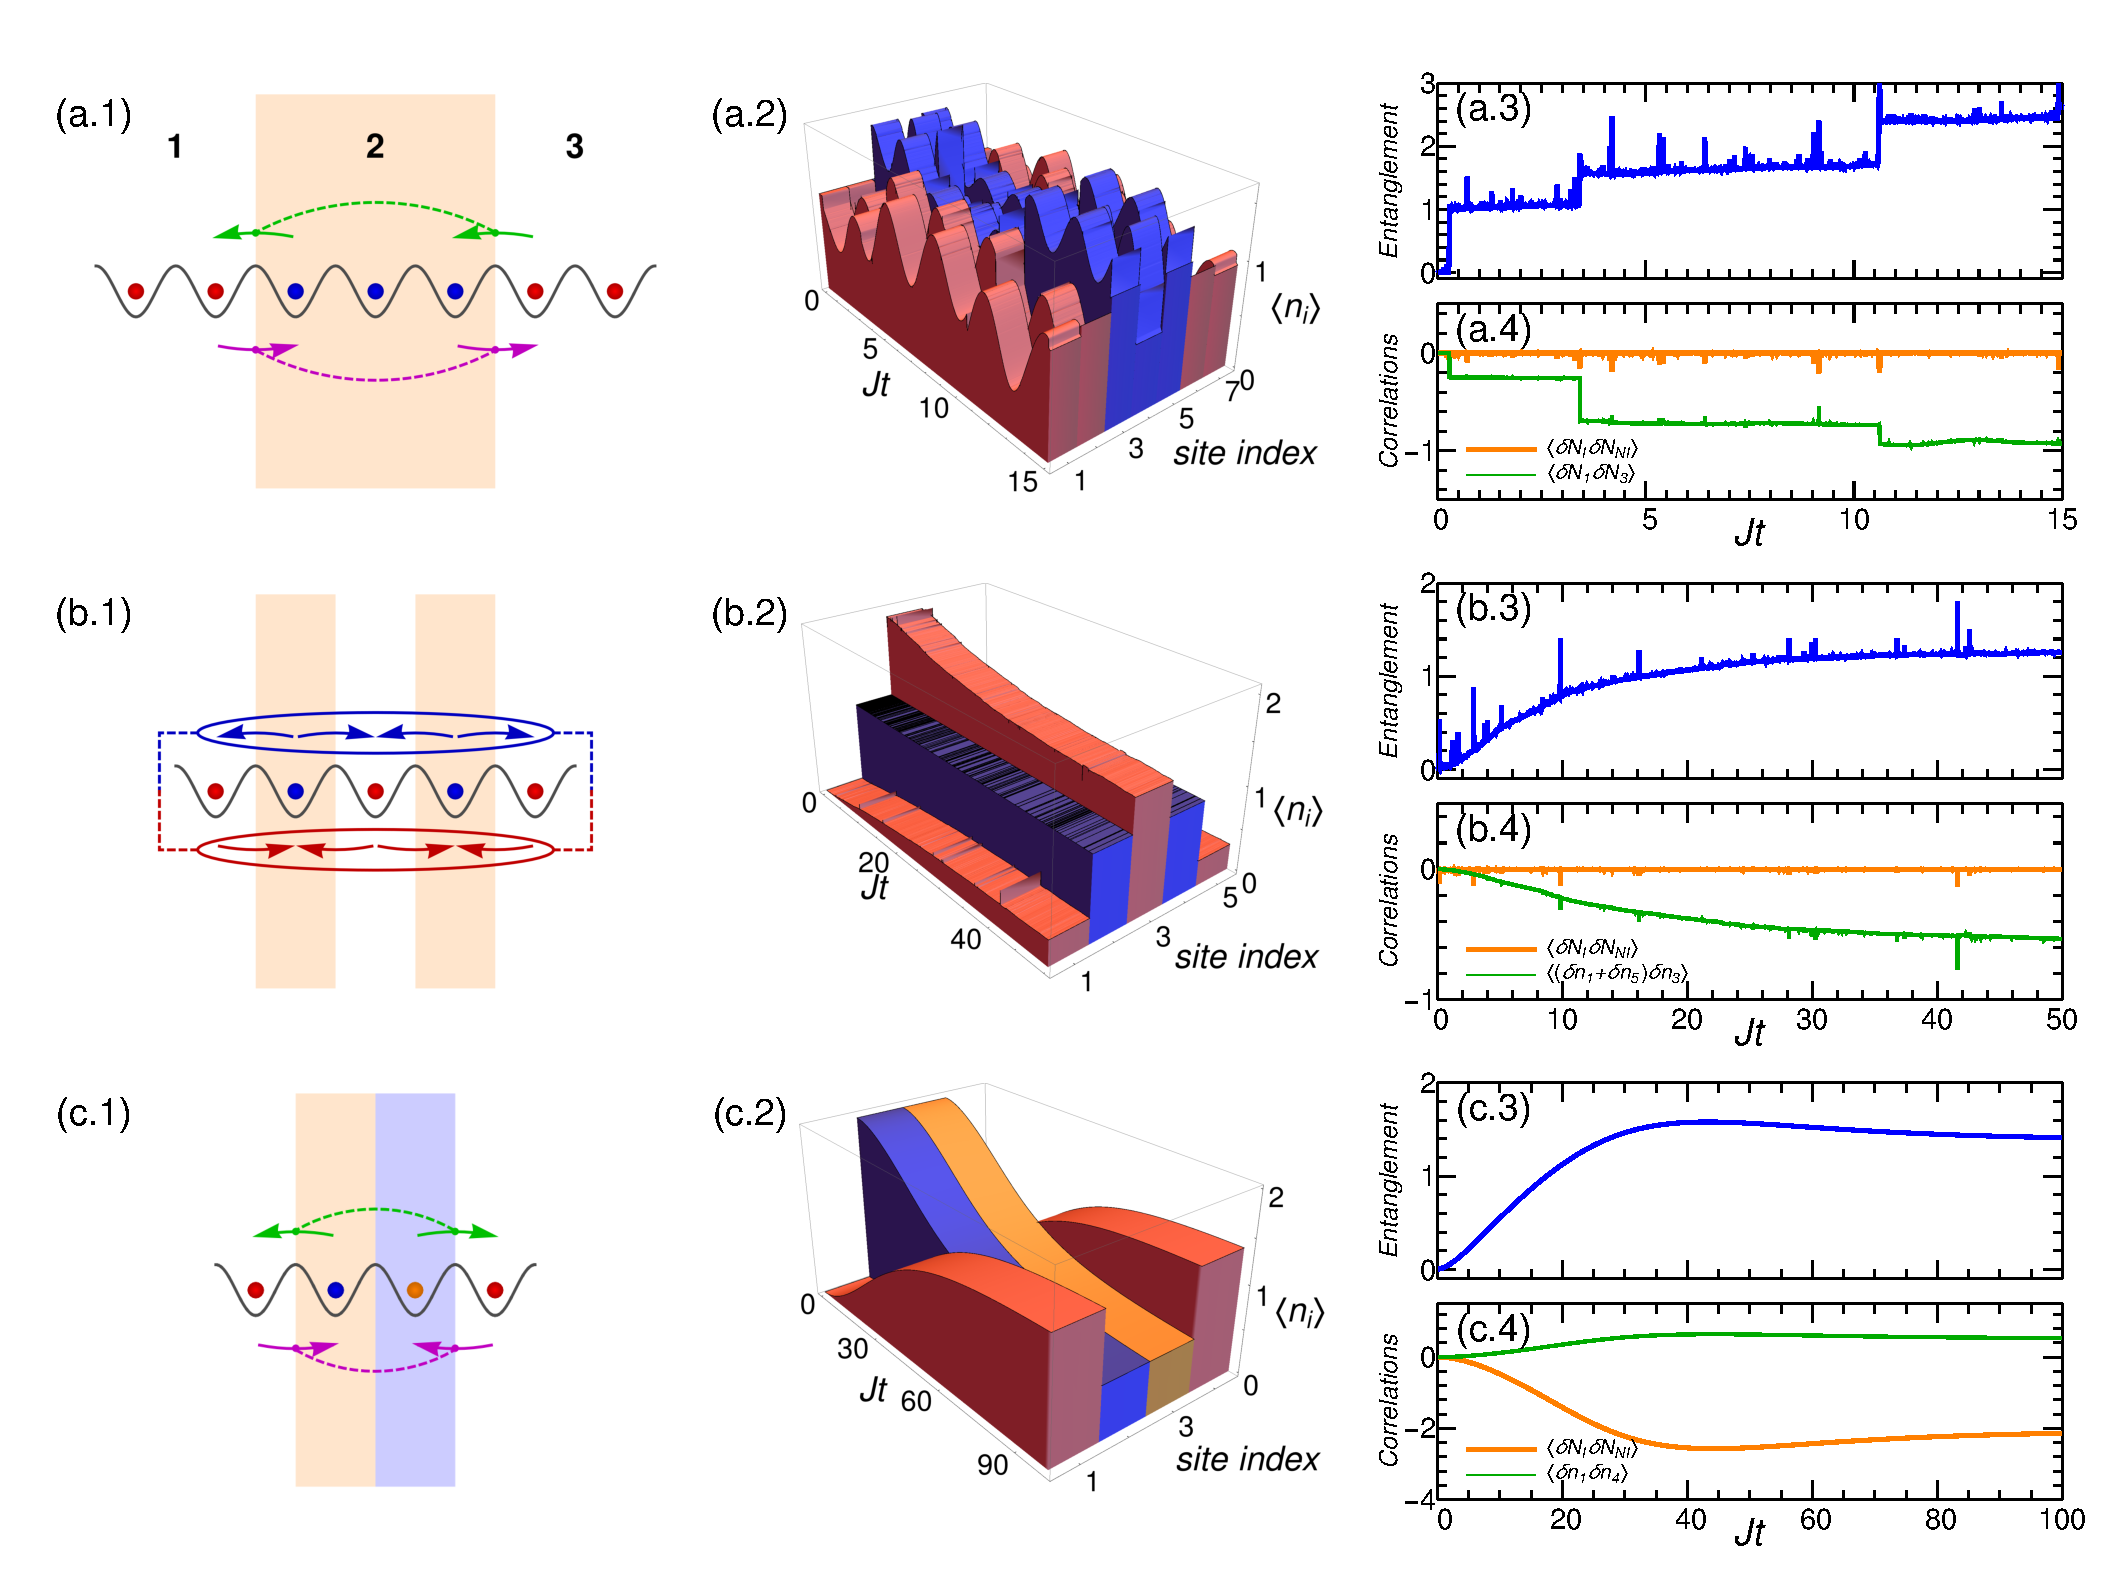
\includegraphics[width=\textwidth]{Zeno.pdf}
  \caption[Emergent Long-Range Correlated Tunnelling]{ Long-range
    correlated tunneling and entanglement, dynamically induced by
    strong global measurement in a single quantum
    trajectory. (a),(b),(c) show different measurement geometries,
    implying different constraints. Panels (1): schematic
    representation of the long-range tunneling processes. Panels (2):
    evolution of on-site densities. Panels (3): entanglement entropy
    growth between illuminated and non-illuminated regions. Panels
    (4): correlations between different modes (orange) and within the
    same mode (green); $N_I$ ($N_{NI}$) is the atom number in the
    illuminated (non-illuminated) mode.  (a) (a.1) Atom number in the
    central region is frozen: system is divided into three
    regions. (a.2) Standard dynamics happens within each region, but
    not between them. (a.3) Entanglement build up. (a.4) Negative
    correlations between non-illuminated regions (green) and zero
    correlations between the $N_I$ and $N_{NI}$ modes
    (orange). Initial state: $|1,1,1,1,1,1,1 \rangle$, $\gamma/J=100$,
    $J_{jj}=[0,0,1,1,1,0,0]$.  (b) (b.1) Even sites are illuminated,
    freezing $N_\text{even}$ and $N_\text{odd}$. Long-range tunneling
    is represented by any pair of one blue and one red arrow. (b.2)
    Correlated tunneling occurs between non-neighbouring sites without
    changing mode populations. (b.3) Entanglement build up. (b.4)
    Negative correlations between edge sites (green) and zero
    correlations between the modes defined by $N_\text{even}$ and
    $N_\text{odd}$ (orange). Initial state: $|0,1,2,1,0 \rangle$,
    $\gamma/J=100$, $J_{jj}=[0,1,0,1,0]$.  (c) (c.1,2) Atom number
    difference between two central sites is frozen. (c.3) Entanglement
    build up. (c.4) In contrast to previous examples, sites in the
    same zones are positively correlated (green), while atoms in
    different zones are negatively correlated (orange). Initial state:
    $|0,2,2,0 \rangle$, $\gamma/J=100$, $J_{jj}=[0,-1,1,0]$. 1D
    lattice, $U/J=0$.}
  \label{fig:zeno}
\end{figure}

There are two crucial features of the resulting dynamics that are of
note. First, just like in the infinite quantum Zeno limit the
evolution between nearest neighbours within the same mode is
unperturbed whilst tunnelling between different modes is heavily
suppressed by the measurement. Therefore, we see the usual quantum
Zeno dynamics within a single Zeno subspace and just like before, it
is also possible to use the global probing scheme to engineer these
eigenspaces and select which tunnelling processes should be
uninhibited and which should be suppressed. However, there is a second
effect that was not present before. In Fig. \ref{fig:zeno} we can
observe tunnelling that violates the boundaries established by the
spatial modes. When $\gamma$ is finite, second-order processes,
i.e.~two correlated tunnelling events, can now occur via an
intermediate (virtual) state outside of the Zeno subspace as long as
the Zeno subspace of the final state remains the same. Crucially,
these tunnelling events are only correlated in time, but not in
space. This means that the two events do not have to occur for the
same atom or even at the same site in the lattice. As long as the Zeno
subspace is preserved, these processes can occur anywhere in the
system. That is, a pair of atoms separated by many sites is able to
tunnel in a correlated manner. This is only possible due to the
ability of creating extensive and spatially nonlocal modes as
described in section \ref{sec:modes} which in turn is enabled by the
global nature of the measurement. This would not be possible to
achieve with local measurements as the Zeno subspaces would be
described entirely by local variables which cannot be preserved by
such delocalised tunnelling events.

In the subsequent sections we will rigorously derive the following
Hamiltonian for the non-interacting dynamics within a single Zeno
subspace, $\varphi = 0$, for a lattice where the measurement defines
$Z = 2$ distinct modes, e.g. $\hat{D} = \hat{N}_K$ or
$\hat{D} = \hat{N}_\mathrm{odd}$
\begin{equation}
  \label{eq:hz}
  \hat{H}_\varphi = P_0 \left[ -J \sum_{\langle i, j \rangle}
    b^\dagger_i b_j - i \frac{J^2} {A \gamma} \sum_{\varphi} 
    \sum_{\substack{\langle i \in \varphi, j \in \varphi^\prime
        \rangle \\ \langle k \in \varphi^\prime, l \in \varphi
        \rangle}} b^\dagger_i b_j b^\dagger_k b_l \right] P_0,
\end{equation}
where
$A = (J_{\varphi,\varphi} - J_{\varphi^\prime,\varphi^\prime})^2$ is a
constant that depends on the measurement scheme, $\varphi$ denotes a
set of sites belonging to a single mode and $\varphi^\prime$ is the
set's complement (e.g.~odd and even or illuminated and non-illuminated
sites). We see that this Hamiltonian consists of two parts. The first
term corresponds to the standard quantum Zeno first-order dynamics
that occurs within a Zeno subspace, i.e.~tunnelling between
neighbouring sites that belong to the same mode. Otherwise, if $i$ and
$j$ belong to different modes $P_0 \bd_i b_j P_0 = 0$. When
$\gamma \rightarrow \infty$ we recover the quantum Zeno Hamiltonian
where this would be the only remaining term. It is the second term
that shows the second-order corelated tunnelling terms. This is
evident from the inner sum which requires that pairs of sites ($i$,
$j$) and ($k$, $l$) between which atoms tunnel must be nearest
neighbours, but these pairs can be anywhere on the lattice within the
constraints of the mode structure. This is in particular explicitly
shown in Figs. \ref{fig:zeno}(a,b). The imaginary coefficient means
that the tinelling behaves like an exponential decay (overdamped
oscillations). This also implies that the norm will decay, but this
does not mean that there are physical losses in the system. Instead,
the norm itself represents the probability of the system remaining in
the $\varphi = 0$ Zeno subspace. Since $\gamma$ is not infinite there
is now a finite probability that the stochastic nature of the
measurement will lead to a discontinous change in the system where the
Zeno subspace rapidly changes which can be seen in
Fig. \ref{fig:zeno}(a). However, later in this chapter we will see
that steady states of this Hamiltonian exist which will no longer
change Zeno subspaces.

Crucially, what sets this effect apart from usual many-body dynamics
with short-range interactions is that first order processes are
selectively suppressed by the global conservation of the measured
observable and not by the prohibitive energy costs of doubly-occupied
sites, as is the case in the $t$-$J$ model \cite{auerbach}. This has
profound consequences as this is the physical origin of the long-range
correlated tunneling events represented in Eq. \eqref{eq:hz} by the
fact that the pairs ($i$, $j$) and ($k$, $l$) can be very distant. The
projection $\hat{P}_0$ is not sensitive to individual site
occupancies, but instead enforces a fixed value of the observable,
i.e.~a single Zeno subspace. This is a striking difference with the
$t$-$J$ and other strongly interacting models. The strong interaction
also leads to correlated events in which atoms can tunnel over each
other by creating an unstable doubly occupied site during the
intermediate step. However, these correlated events are by their
nature localised. Due to interactions the doubly-occupied site cannot
be present in the final state which means that any tunnelling event
that created this unstable configuration must be followed by another
tunnelling event which takes an atom away. In the case of global
measurement this process is delocalised, because since the modes
consist of many sites the stable configuration can be restored by a
tunnelling event from a completely different lattice site that belongs
to the same mode.

In Fig.~\ref{fig:zeno}a we consider illuminating only the central
region of the optical lattice and detecting light in the diffraction
maximum, thus we freeze the atom number in the $K$ illuminated sites
$\hat{N}_\text{K}$~\cite{mekhov2009prl,mekhov2009pra}. The measurement
scheme defines two different spatial modes: the non-illuminated zones
$1$ and $3$ and the illuminated one $2$. Figure~\ref{fig:zeno}(a.2)
illustrates the evolution of the mean density at each lattice site:
typical dynamics occurs within each region but the standard tunnelling
between different modes is suppressed. Importantly, second-order
processes that do not change $N_\text{K}$ are still possible since an
atom from $1$ can tunnel to $2$, if simultaneously one atom tunnels
from $2$ to $3$. Therefore, effective long-range tunneling between two
spatially disconnected zones $1$ and $3$ happens due to the two-step
processes $1 \rightarrow 2 \rightarrow 3$ or
$3 \rightarrow 2 \rightarrow 1$. These transitions are responsible for
the negative (anti-)correlations
$\langle \delta N_1 \delta N_3 \rangle = \langle N_1 N_3 \rangle -
\langle N_1 \rangle \langle N_3 \rangle$ showing that an atom
disappearing from zone $1$ appears in zone $3$, while there are no
number correlations between illuminated and non-illuminated regions,
$\langle( \delta N_1 + \delta N_3 ) \delta N_2 \rangle = 0$ as shown
in Fig.~\ref{fig:zeno}(a.4). In contrast to fully-projective
measurement, the existence of an intermediate (virtual) step in the
correlated tunnelling process builds long-range entanglement between
illuminated and non-illuminated regions as shown in
Fig.~\ref{fig:zeno}(a.3).

To make correlated tunneling visible even in the mean atom number, we
suppress the standard Bose-Hubbard dynamics by illuminating only the
even sites of the lattice in Fig.~\ref{fig:zeno}(b). Even though this
measurement scheme freezes both $N_\text{even}$ and $N_\text{odd}$,
atoms can slowly tunnel between the odd sites of the lattice, despite
them being spatially disconnected. This atom exchange spreads
correlations between non-neighbouring lattice sites on a time scale
$\sim \gamma/J^2$ as seen in Eq. \eqref{eq:hz}. The schematic
explanation of long-range correlated tunneling is presented in
Fig.~\ref{fig:zeno}(b.1): the atoms can tunnel only in pairs to assure
the globally conserved values of $N_\text{even}$ and $N_\text{odd}$,
such that one correlated tunneling event is represented by a pair of
one red and one blue arrow. Importantly, this scheme is fully
applicable for a lattice with large atom and site numbers, well beyond
the numerical example in Fig.~\ref{fig:zeno}(b.1), because as we can
see in Eq. \eqref{eq:hz} it is the geometry of quantum measurement that
assures this mode structure (in this example, two modes at odd and
even sites) and thus the underlying pairwise global tunnelling.

The scheme in Fig.~\ref{fig:zeno}(b.1) can help design a nonlocal
reservoir for the tunneling (or ``decay'') of atoms from one region to
another. For example, if the atoms are placed only at odd sites,
according to Eq. \eqref{eq:hz} their tunnelling is suppressed since the
multi-tunneling event must be successive, i.e.~an atom tunnelling into
a different mode, $\varphi^\prime$, must then also tunnel back into
its original mode, $\varphi$. If, however, one adds some atoms to even
sites (even if they are far from the initial atoms), the correlated
tunneling events become allowed and their rate can be tuned by the
number of added atoms. This resembles the repulsively bound pairs
created by local interactions \cite{winkler2006, folling2007}. In
contrast, here the atom pairs are nonlocally correlated due to the
global measurement. Additionally, these long-range correlations are a
consequence of the dynamics being constrained to a Zeno subspace: the
virtual processes allowed by the measurement entangle the spatial
modes nonlocally. Since the measurement only reveals the total number
of atoms in the illuminated sites, but not their exact distribution,
these multi-tunelling events cause the build-up of long range
entanglement. This is in striking contrast to the entanglement caused
by local processes which can be very confined, especially in 1D where
it is typically short range. This makes numerical calculations of our
system for large atom numbers really difficult, since well-known
methods such as DMRG and MPS \cite{schollwock2005} (which are
successful for short-range interactions) rely on the limited extent of
entanglement.

The negative number correlations are typical for systems with
constraints (superselection rules) such as fixed atom number. The
effective dynamics due to our global, but spatially structured,
measurement introduces more general constraints to the evolution of
the system. For example, in Fig.~\ref{fig:zeno}(c) we show the
generation of positive number correlations shown in
Fig.~\ref{fig:zeno}(c.4) by freezing the atom number difference
between the sites ($N_\text{odd}-N_\text{even}$). Thus, atoms can only
enter or leave this region in pairs, which again is possible due to
correlated tunneling as seen in Figs.~\ref{fig:zeno}(c.1,c.2) and
manifests positive correlations. As in the previous example, two edge
modes in Fig.~\ref{fig:zeno}(c) can be considered as a nonlocal
reservoir for two central sites, where a constraint is applied. Note
that, using more modes, the design of higher-order multi-tunneling
events is possible.

This global pair tunneling may play a role of a building block for
more complicated many-body effects. For example, a pair tunneling
between the neighbouring sites has been recently shown to play
important role in the formation of new quantum phases, e.g., pair
superfluid \cite{sowinski2012} and lead to formulation of extended
Bose-Hubbard models \cite{omjyoti2015}. The search for novel
mechanisms providing long-range interactions is crucial in many-body
physics. One of the standard candidates is the dipole-dipole
interaction in, e.g., dipolar molecules, where the mentioned pair
tunneling between even neighboring sites is already considered to be
long-range \cite{sowinski2012,omjyoti2015}. In this context, our work
suggests a fundamentally different mechanism originating from quantum
optics: the backaction of global and spatially structured measurement,
which as we prove can successfully compete with other short-range
processes in many-body systems. This opens promising opportunities for
future research.

\section{Non-Hermitian Dynamics in the Quantum Zeno Limit}

In the previous section we provided a rather high-level analysis of
the strong measurement limit in our quantum gas model. We showed that
global measurement in the strong, but not projective, limit leads to
correlated tunnelling events which can be highly delocalised. Multiple
examples for different optical geometries and measurement operators
demonstrated the incredible felixbility and potential in engineering
dynamics for ultracold gases in an optical lattice. We also claimed
that the behaviour of the system is described by the Hamiltonian given
in Eq. \eqref{eq:hz}. Having developed a physical and intuitive
understanding of the dynamics in the quantum Zeno limit we will now
provide a more rigorous, low-level and fundamental understanding of
the process.

\subsection{Suppression of Coherences in the Density Matrix}

At this point we deviate from the quantum trajectory approach and we
resort to a master equation as introduced in section
\ref{sec:master}. We do this, because we have seen that the emergent
long-range correlated tunnelling is a feature of all trajectories and
mostly depends on the geometry of the measurement. Therefore, a
general approach starting from an unconditioned state should be able
to reveal these features. However, we will later make use of the fact
that we are in possession of a measurement record and obtain a
conditioned state. Furthermore, we first consider the most general
case of an open system subject to a quantum measurement and only limit
ourselves to the quantum gas model later on. This demonstrates that
the dynamics we observed in the previous section are a feature of
measurement rather than our specific model.

As introduced in section \ref{sec:master} we consider a state
described by the density matrix $\hat{\rho}$ whose isolated behaviour
is described by the Hamiltonian $\H_0$ and when measured the jump
operator $\c$ is applied to the state at each detection
\cite{MeasurementControl}. The master equation describing its time
evolution when we ignore the measurement outcomes is given by
\begin{equation}
  \dot{\hat{\rho}} = -i [ \H_0 , \hat{\rho} ] + \c \hat{\rho} \cd - \frac{1}{2}(
  \cd\c \hat{\rho} + \hat{\rho} \cd\c ).
\end{equation}
We also define $\c = \lambda \op$ and $\H_0 = \nu \h$. The exact
definition of $\lambda$ and $\nu$ is not so important as long as these
coefficients can be considered to be some measure of the relative size
of these operators. They would have to be determined on a case-by-case
basis, because the operators $\c$ and $\H_0$ may be unbounded. If
these operators are bounded, one can simply define them such that
$||\op|| \sim O(1)$ and $||\h|| \sim O(1)$. If they are unbounded, one
possible approach would be to identify the relevant subspace of which
dynamics we are interested in and scale the operators such that the
eigenvalues of $\op$ and $\h$ in this subspace are $\sim O(1)$.

We will once again use projectors $P_m$ which have no effect on states
within a degenerate subspace of $\c$ ($\op$) with eigenvalue $c_m$
($o_m$), but annihilate everything else. For convenience we will also
use the following definition $\hat{\rho}_{mn} = P_m \hat{\rho} P_n$.
Note that these are submatrices of the density matrix, which in
general are not single matrix elements. Therefore, we can write the
master equation that describes this open system as a set of equations
\begin{equation}
\label{eq:master}
  \dot{\hat{\rho}}_{mn} =  -i K P_m \left[ \h \sum_r \hat{\rho}_{rn}
    - \sum_r \hat{\rho}_{mr} \h \right] P_n + \lambda^2 \left[ o_m
    o_n^*  - \frac{1}{2} \left( |o_m|^2 + |o_n|^2 \right) \right] \hat{\rho}_{mn},
\end{equation}
where the first term describes coherent evolution whereas the second
term causes dissipation. 

First, note that for the density submatrices for which $m = n$,
$\hat{\rho}_{mm}$, the dissipative term vanishes. This means that
these submatrices are subject to coherent evolution only and do not
experience losses and they are thus decoherence free subspaces. It is
crucial to note that these submatrices are simply the density matrices
of the individual degenerate Zeno subspaces. Interestingly, any state
that consists only of these decoherence free subspaces, i.e.~
$\hat{\rho} = \sum_m \hat{\rho}_{mm}$, and that commutes with the
Hamiltonian, $[\hat{\rho}, \hat{H}_0] = 0$, will be a steady state.
This can be seen by substituting this ansatz into
Eq. \eqref{eq:master} which yields $\dot{\hat{\rho}}_{mn} = 0$ for all
$m$ and $n$. These states can be prepared dissipatively using known
techniques \cite{diehl2008}, but it is not required that the state be
a dark state of the dissipative operator as is usually the case.

Second, we consider a large detection rate, $\lambda^2 \gg \nu$, for
which the coherences, i.e.~ the density submatrices $\hat{\rho}_{mn}$
for which $m \ne n$, will be heavily suppressed by dissipation. We can
adiabatically eliminate these cross-terms by setting
$\dot{\hat{\rho}}_{mn} = 0$, to get
\begin{equation}
\label{eq:intermediate}
\hat{\rho}_{mn} = \frac{\nu}{\lambda^2} \frac{i P_m \left[ \h \sum_r \hat{\rho}_{rn} - \sum_r \hat{\rho}_{mr} \h \right] P_n } {o_m o_n^* - \frac{1}{2} \left( |o_m|^2 + |o_n|^2 \right)}
\end{equation}
which tells us that they are of order $\nu/\lambda^2 \ll
1$. Therefore, the resulting density matrix will be given by
$\hat{\rho} \approx \sum_m \hat{\rho}_{mm}$ which consists solely of
the individual Zeno subspace density matrices. One can easily recover
the projective Zeno limit by considering $\lambda \rightarrow \infty$
when all the subspaces completely decouple. This is exactly the
$\gamma \rightarrow \infty$ limit discussed in the previous
section. However, we have seen that it is crucial we only consider,
$\lambda^2 \gg \nu$, but not infinite. If the subspaces do not
decouple completely, then transitions within a single subspace can
occur via other subspaces in a manner similar to Raman transitions. In
Raman transitions population is transferred between two states via a
third, virtual, state that remains empty throughout the process. By
avoiding the infinitely projective Zeno limit we open the option for
such processes to happen in our system where transitions within a
single Zeno subspace occur via a second, different, Zeno subspace even
though the occupation of the intermediate states will remian
negligible at all times.

A single quantum trajectory results in a pure state as opposed to the
density matrix and in general, there are many density matrices that
have non-zero and non-negligible $m = n$ submatrices,
$\hat{\rho}_{mm}$, even when the coherences are small. They correspond
to a mixed states containing many Zeno subspaces and it is not clear
what the pure states that make up these density matrices are. However,
we note that for a single pure state the density matrix can consist of
only a single diagonal submatrix $\hat{\rho}_{mm}$. To understand
this, consider the state $| \Phi \rangle$ and take it to span exactly
two distinct subspaces $P_a$ and $P_b$ ($a \ne b$). This wavefunction
can thus be written as
$| \Phi \rangle = P_a | \Phi \rangle + P_b | \Phi \rangle$. The
corresponding density matrix is given by
\begin{equation}
  \hat{\rho}_\Psi = P_a | \Phi \rangle \langle \Phi | P_a + P_a | \Phi
  \rangle \langle \Phi | P_b + P_b | \Phi \rangle \langle \Phi | P_a +
  P_b | \Phi \rangle \langle \Phi | P_b.
\end{equation}
If the wavefunction has significant components in both subspaces then
in general the density matrix will not have negligible coherences,
$\hat{\rho}_{ab} = P_a | \Phi \rangle \langle \Phi | P_b$. A density
matrix with just diagonal components must be in either subspace $a$,
$| \Phi \rangle = P_a | \Phi \rangle$, or in subspace $b$,
$| \Phi \rangle = P_b | \Phi \rangle$. Therefore, a density matrix of
the form $\hat{\rho} = \sum_m \hat{\rho}_{mm}$ without any cross-terms
between different Zeno subspaces can only be composed of pure states
that each lie predominantly within a single subspace. However, because
we will not be dealing with the projective limit, the wavefunction
will in general not be entirely confined to a single Zeno subspace. We
have seen that the coherences are of order $\nu/\lambda^2$. This would
require the wavefunction components to satisfy
$P_a | \Phi \rangle \approx O(1)$ and
$P_b | \Phi \rangle \approx O(\nu/\lambda^2)$ (or vice-versa). This in
turn implies that the population of the states outside of the dominant
subspace (and thus the submatrix $\hat{\rho}_{bb}$) will be of order
$\langle \Phi | P_b^2 | \Phi \rangle \approx
O(\nu^2/\lambda^4)$. Therefore, these pure states, even though they
span multiple Zeno subspaces, cannot exist in a meaningful coherent
superposition in this limit. This means that a density matrix that
spans multiple Zeno subspaces has only classical uncertainty about
which subspace is currently occupied as opposed to the uncertainty due
to a quantum superposition. This is anlogous to the simple qubit
example we considered in section \ref{sec:master}.
 
\subsection{Quantum Measurement vs. Dissipation}

This is where quantum measurement deviates from dissipation. If we
have access to a measurement record we can infer which Zeno subspace
is occupied, because we know that only one of them can be occupied at
any time. We have seen that since the density matrix cross-terms are
small we know \emph{a priori} that the individual wavefunctions
comprising the density matrix mixture will not be coherent
superpositions of different Zeno subspaces and thus we only have
classical uncertainty which means we can resort to clasical
probability methods. Each individual experiment will at any time be
predominantly in a single Zeno subspace with small cross-terms and
negligible occupations in the other subspaces. With no measurement
record our density matrix would be a mixture of all these
possibilities. We can try and determine the Zeno subspace around which
the state evolves in a single experiment from the number of
detections, $m$, in time $t$.

The detection distribution on time-scales shorter than dissipation (so
we can approximate as if we were in a fully Zeno regime) can be
obtained by integrating over the detection times \cite{mekhov2009pra}
to get
\begin{equation}
  P(m,t) = \sum_n \frac{[|c_n|^2 t]^m} {m!} e^{-|c_n|^2 t} \mathrm{Tr} (\rho_{nn}).
\end{equation}
For a state that is predominantly in one Zeno subspace, the
distribution will be approximately Poissonian (up to
$O(\nu^2 / \lambda^4)$, the population of the other
subspaces). Therefore, in a single experiment we will measure
$m = |c_0|^2t \pm \sqrt{|c_0|^2t}$ detections (note, we have assumed
$|c_0|^2 t$ is large enough to approximate the distribution as
normal. This is not necessary, we simply use it here to not have to
worry about the asymmetry in the deviation around the mean value). The
uncertainty does not come from the fact that $\lambda$ is not
infinite. The jumps are random events with a Poisson
distribution. Therefore, even in the full projective limit we will not
observe the same detection trajectory in each experiment even though
the system evolves in exactly the same way and remains in a perfectly
pure state.

If the basis of $\c$ is continuous (e.g. free particle position or
momentum) then the deviation around the mean will be our upper bound
on the deviation of the system from a pure state evolving around a
single Zeno subspace. However, continuous systems are beyond the scope
of this work and we will confine ourselves to discrete systems. Though
it is important to remember that continuous systems can be treated
this way, but the error estimate (and thus the mixedness of the state)
will be different.

For a discrete system it is easier to exclude all possibilities except
for one. The error in our estimate of $|c_0|^2$ in a single experiment
decreases as $1/\sqrt{t}$ and thus it can take a long time to
confidently determine $|c_0|^2$ to a sufficient precision this
way. However, since we know that it can only take one of the possible
values from the set $\{|c_n|^2 \}$ it is much easier to instead
exclude all the other values.

In an experiment we can use Bayes' theorem to infer the state of our
system as follows
\begin{equation}
	p(c_n = c_0 | m) = \frac{ p(m | c_n = c_0) p(c_n = c_0) }{ p(m) },
\end{equation}
where $p(x)$ denotes the probability of the discrete event $x$ and
$p(x|y)$ the conditional probability of $x$ given $y$. We know that
$p(m | c_n = c_0)$ is simply given by a Poisson distribution with mean
$|c_0|^2 t$. $p(m)$ is just a normalising factor and $p(c_n = c_0)$ is
our \emph{a priori} knowledge of the state. Therefore, one can get the
probability of being in the right Zeno subspace from
\begin{align}
  p(c_n & = c_0 | m) = \frac{ p_0(c_n = c_0) \frac{ \left( |c_0|^2 t
          \right)^{2m} } {m!} e^{-|c_0|^2 t}} {\sum_n p_0(c_n) \frac{
          \left( |c_n|^2 t \right)^{2m} } {m!} e^{-|c_n|^2 t}} \nonumber \\
	& = p_0(c_n = c_0) \left[ \sum_n p_0(c_n) \left( \frac{
          |c_n|^2 } { |c_0|^2 } \right)^{2m} e^{\left( |c_0|^2 -
          |c_n|^2 \right) t} \right]^{-1},
\end{align}
where $p_0$ denotes probabilities at $t = 0$. In a real experiment one
could prepare the initial state to be close to the Zeno subspace of
interest and thus it would be easier to deduce the state. Furthermore,
in the middle of an experiment if we have already established the Zeno
subspace this will be reflected in these \emph{a priori} probabilities
again making it easier to infer the correct subspace. However, we will
consider the worst case scenario which might be useful if we don't
know the initial state or if the Zeno subspace changes during the
experiment, a uniform $p_0(c_n)$.

This probability is a rather complicated function as $m$ is a
stochastic quantity that also increases with $t$. We want it to be as
close to $1$ as possible. In order to devise an appropriate condition
for this we note that in the first line all terms in the denominator
are Poisson distributions of $m$. Therefore, if the mean values
$|c_n|^2 t$ are sufficiently spaced out, only one of the terms in the
sum will be significant for a given $m$ and if this happens to be the
one that corresponds to $c_0$ we get a probability close to
unity. Therefore, we set the condition such that it is highly unlikely
that our measured $m$ could be produced by two different distributions
\begin{align}
  \sqrt{|c_0|^2 t} \ll ||c_0|^2 - |c_n|^2| t, \forall n \ne 0 \\
  \sqrt{|c_n|^2 t} \ll ||c_0|^2 - |c_n|^2| t, \forall n \ne 0
\end{align}
The left-hand side is the standard deviation of $m$ if the system was
in subspace $P_0$ or $P_n$. The right-hand side is the difference in
the mean detections between the subspace $n$ and the one we are
interested in. The condition becomes more strict if the subspaces
become less distinguishable as it becomes harder to confidently
determine the correct state. Once again, using $\c = \lambda \hat{o}$
where $\hat{o} \sim O(1)$ we get
\begin{equation}
  t \gg \frac{1}{\lambda^2} \frac{|o_{0,n}|^2} {(|o_0|^2 - |o_n|^2|)^2}.
\end{equation}
Since detections happen on average at an average rate of order
$\lambda^2$ we only need to wait for a few detections to satisfy this
condition. Therefore, we see that even in the worst case scenario of
complete ignorance of the state of the system we can very easily
determine the correct subspace. Once it is established for the first
time, the \emph{a priori} information can be updated and it will
become even easier to monitor the system.

However, it is important to note that physically once the quantum
jumps deviate too much from the mean value the system is more likely
to change the Zeno subspace (due to measurement backaction) and the
detection rate will visibly change. Therefore, if we observe a
consistent detection rate it is extremely unlikely that it can be
produced by two different Zeno subspaces so in fact it is even easier
to determine the correct state, but the above estimate serves as a
good lower bound on the necessary detection time.

Having derived the necessary conditions to confidently determine which
Zeno subspace is being observed in the experiment we can make another
approximation thanks to measurement which would be impossible in a
purely dissipative open system. If we observe a number of detections
consistent with the subspace $P_m = P_0$ we can set
$\hat{\rho}_{mn} \approx 0$ for all cases when both $m \ne 0$ and
$n \ne 0$ leaving our density matrix in the form
\begin{equation}
  \label{eq:approxrho}
  \hat{\rho} = \hat{\rho}_{00} + \sum_{r\ne0} (\hat{\rho}_{0r} +
  \hat{\rho}_{r0}).
\end{equation}
We can do this, because the other states are inconsistent with the
measurement record. We know from the previous section that the system
must lie predominantly in only one of the Zeno subspaces and when that
is the case, $\hat{\rho}_{0r} \approx O(\nu/\lambda^2)$ and for
$m \ne 0$ and $n \ne 0$ we have
$\hat{\rho}_{mn} \approx O(\nu^2/\lambda^4)$. Therefore, this amounts
to keeping first order terms in $\nu/\lambda^2$ in our approximation.

This is a crucial step as all $\hat{\rho}_{mm}$ matrices are
decoherence free subspaces and thus they can all coexist in a mixed
state decreasing the purity of the system without
measurement. Physically, this means we exclude trajectories in which
the Zeno subspace has changed (measurement isn't fully projective). By
substituting Eq. \eqref{eq:intermediate} into Eq. \eqref{eq:master} we
see that this happens at a rate of $\nu^2 / \lambda^2$. However, since
the two measurement outcomes cannot coexist any transition between
them happens in discrete transitions (which we know about from the
change in the detection rate as each Zeno subspace will correspond to
a different rate) and not as continuous coherent evolution. Therefore,
we can postselect in a manner similar to Refs. \cite{otterbach2014,
  lee2014prx, lee2014prl}, but our requirements are significantly more
relaxed - we do not require a specific single trajectory, only that it
remains within a Zeno subspace. Furthermore, upon reaching a steady
state, these transitions become impossible as the coherences
vanish. This approximation is analogous to optical Raman transitions
where the population of the excited state is neglected. Here, we can
make a similar approximation and neglect all but one Zeno subspace
thanks to the additional knowledge we gain from knowing the
measurement outcomes.

\subsection{The Non-Hermitian Hamiltonian}

Rewriting the master equation using $\c = c_0 + \delta \c$, where
$c_0$ is the eigenvalue corresponding to the eigenspace defined by the
projector $P_0$ which we used to obtain the density matrix in
Eq. \eqref{eq:approxrho}, we get
\begin{equation}
  \label{eq:finalrho}
  \dot{\hat{\rho}} = -i \left( \H_\mathrm{eff} \hat{\rho} - \hat{\rho}
  \H_\mathrm{eff}^\dagger \right) + \delta \c \hat{\rho} \delta \cd,
\end{equation}
\begin{equation}
  \label{eq:Ham}
  \H_\mathrm{eff} = \H_0 + i \left( c_0^*\c - \frac{|c_0|^2}{2} - \frac{\cd\c}{2} \right).
\end{equation}
The first term in Eq. \eqref{eq:finalrho} describes coherent evolution
due to the non-Hermitian Hamiltonian $\H_\mathrm{eff}$ and the second
term is decoherence due to our ignorance of measurement outcomes. When
we substitute our approximation of the density matrix
$\hat{\rho} = \hat{\rho}_{00} + \sum_{r\ne0} (\hat{\rho}_{0r} +
\hat{\rho}_{r0})$ into Eq. \eqref{eq:finalrho}, the last term
vanishes, $\delta \c \hat{\rho} \delta \cd = 0$. This happens, because
$\delta \c P_0 \hat{\rho} = \hat{\rho} P_0 \delta \c^\dagger = 0$. The
projector annihilates all states except for those with eigenvalue
$c_0$ and so the operator $\delta \c = \c - c_0$ will always evaluate
to $c_0 - c_0 = 0$. Recall that we defined
$\hat{\rho}_{mn} = P_m \hat{\rho} P_n$ which means that every term in
our approximate density matrix contains the projector $P_0$. However,
it is important to note that this argument does not apply to other
second order terms in the master equation, because some terms only
have the projector $P_0$ applied from one side,
e.g.~$\hat{\rho}_{0m}$. The term $\delta \c \hat{\rho} \delta \cd$
applies the fluctuation operator from both sides so it does not matter
in this case, but it becomes relevant for terms such as
$\delta \cd \delta \c \hat{\rho}$. It is important to note that this
term does not automatically vanish, but when the explicit form of our
approximate density matrix is inserted, it is in fact zero. Therefore,
we can omit this term using the information we gained from
measurement, but keep other second order terms, such as
$\delta \cd \delta \c \rho$ in the Hamiltonian which are the origin of
other second-order dynamics. This could not be the case in a
dissipative system.

Ultimately we find that a system under continuous measurement for
which $\lambda^2 \gg \nu$ in the Zeno subspace $P_0$ is described by
the deterministic non-Hermitian Hamiltonian $\H_\mathrm{eff}$ in
Eq. \eqref{eq:Ham} and thus obeys the following Schr\"{o}dinger
equation
\begin{equation}
 i \frac{\mathrm{d} | \Psi \rangle}{\mathrm{d}t} = \left[\H_0 + i \left(
      c_0^*\c - \frac{|c_0|^2}{2} - \frac{\cd\c}{2} \right) \right] |
  \Psi \rangle.
\end{equation}
Of the three terms in the parentheses the first two represent the
effects of quantum jumps due to detections (which one can think of as
`reference frame' shifts between different degenerate eigenspaces) and
the last term is the non-Hermitian decay due to information gain from
no detections. It is important to emphasize that even though we
obtained a deterministic equation, we have not neglected the
stochastic nature of the detection events. The detection trajectory
seen in an experiment will have fluctuations around the mean
determined by the Zeno subspace, but there simply are many possible
measurement records with the same outcome. This is just like the fully
projective Zeno limit where the system remains perfectly pure in one
of the possible projections, but the detections remain randomly
distributed in time.

One might then be concerned that purity is preserved even though we
might be averaging over many trajectories within this Zeno
subspace. We have neglected the small terms $\hat{\rho}_{m,n}$
($m,n \ne 0$) which are $O(\nu^2/\lambda^4)$ and thus they are not
correctly accounted for by our approximation. This means that we have
an $O(\nu^2/\lambda^4)$ error in our density matrix. The purity
given by
\begin{equation}
  \mathrm{Tr}(\hat{\rho}^2) = \mathrm{Tr}(\hat{\rho}^2_{00} + \sum_{m \ne
    0} \hat{\rho}_{0m}\hat{\rho}_{m0}) + \mathrm{Tr}(\sum_{m,n\ne0}
  \hat{\rho}_{mn} \hat{\rho}_{nm})
\end{equation}
where the second term contains the terms not accounted for by our
approximation thus introduces an $O(\nu^4/\lambda^8)$
error. Therefore, this discrepancy is negligible in our
approximation. The pure state predicted by $\H_\mathrm{eff}$ is only
an approximation, albeit a good one, and the real state will be mixed
to a small extent. Whilst perfect purity within the Zeno subspace
$\hat{\rho}_{00}$ is expected due to the measurement's strong
decoupling effect, the nearly perfect purity when transitions outside
the Zeno subspace are included is a nontrivial result. Similarly, in
Raman transitions the population of the neglected excited state is
also non-zero, but negligible. Furthermore, this equation does not
actually require the adiabatic elimination used in
Eq. \eqref{eq:intermediate} (we only used it to convince ourselves
that the coherences are small) and such situations may be considered
provided all approximations remain valid. In a similar way the limit
of linear optics is derived from the physics of a two-level nonlinear
medium, when the population of the upper state is neglected and the
adiabatic elimination of coherences is not required.

\subsection{Non-Hermitian Dynamics in Ultracold Gases}

We finally return to our quantum gas model inside of a cavity. We
start by considering the simplest case of a global multi-site
measurement of the form $\hat{D} = \hat{N}_K = \sum_i^K \n_i$, where
the sum is over $K$ illuminated sites. The effective Hamiltonian
becomes
\begin{equation}
  \label{eq:nHH2}
  \hat{H}_\mathrm{eff} = \hat{H}_0 - i \gamma \left(  \delta \hat{N}_K \right)^2,
\end{equation}
where $ \delta \hat{N}_K = \hat{N}_K - N^0_K$ and $N^0_K$ is the Zeno
subspace eigenvalue. It is now obvious that continuous measurement
squeezes the fluctuations in the measured quantity, as expected, and
that the only competing process is the system's own dynamics.

In this case, if we adiabatically eliminate the density matrix
cross-terms and substitute Eq. \eqref{eq:intermediate} into
Eq. \eqref{eq:master} for this system we obtain an effective
Hamiltonian within the Zeno subspace defined by $N_K$
\begin{equation}
  \H_\varphi = P_0 \left[ \H_0 - i \frac{J^2}{\gamma}
    \sum_\varphi \sum_{\substack{\langle i \in \varphi, j \in \varphi^\prime
        \rangle \\ \langle k \in \varphi^\prime, l \in \varphi
        \rangle}} b^\dagger_i b_j b^\dagger_k b_l \right] P_0,
\end{equation}
where $\varphi$ denotes a set of sites belonging to a single mode and
$\varphi^\prime$ is the set's complement (e.g. odd and even or
illuminated and non-illuminated sites) and $P_0$ is the projector onto
the eigenspace with $N_K^0$ atoms in the illuminated area. We focus on
the case when the second term is not only significant, but also leads
to dynamics within a Zeno subspace that are not allowed by
conventional quantum Zeno dynamics accounted for by the first
term. The second term represents second-order transitions via other
subspaces which act as intermediate states much like virtual states in
optical Raman transitions. This is in contrast to the conventional
understanding of the Zeno dynamics for infinitely frequent projective
measurements (corresponding to $\gamma \rightarrow \infty$) where such
processes are forbidden \cite{facchi2008}. Thus, it is the weak
quantum measurement that effectively couples the states. Note that
this is a special case of the equation in Eq. \eqref{eq:hz} which can
be obtained by considering a more general two mode setup.

\subsection{Small System Example}

To get clear physical insight, we initially consider three atoms in
three sites and choose our measurement operator such that
$\hat{D} = \n_2$, i.e.~only the middle site is subject to measurement,
and the Zeno subspace defined by $n_2 = 1$. Such an illumination
pattern can be achieved with global addressing by crossing two beams
and placing the nodes at the odd sites and the antinodes at even
sites. This means that $P_0 \H_0 P_0 = 0$. However, the
first and third sites are connected via the second term. Diagonalising
the Hamiltonian reveals that out of its ten eigenvalues all but three
have a significant negative imaginary component of the order $\gamma$
which means that the corresponding eigenstates decay on a time scale
of a single quantum jump and thus quickly become negligible. The three
remaining eigenvectors are dominated by the linear superpositions of
the three Fock states $|2,1,0 \rangle$, $|1, 1, 1 \rangle$, and
$|0,1,2 \rangle$. Whilst it is not surprising that these components
are the only ones that remain as they are the only ones that actually
lie in the Zeno subspace $n_2 = 1$, it is impossible to solve the full
dynamics by just considering these Fock states alone as they are not
coupled to each other in $\hat{H}_0$. The components lying outside of
the Zeno subspace have to be included to allow intermediate steps to
occur via states that do not belong in this subspace, much like
virtual states in optical Raman transitions.

An approximate solution for $U=0$ can be written for the
$\{|2,1,0 \rangle, |1,1,1 \rangle, |0,1,2 \rangle\}$ subspace by
multiplying each eigenvector with its corresponding time evolution
\begin{equation}
  | \Psi(t) \rangle \propto \left( \begin{array}{c} 
  z_1 + \sqrt{2} z_2 e^{-6 J^2 t / \gamma} + z_3 e^{-12 J^2 t / \gamma} \\
  -\sqrt{2} \left(z_1 - z_3 e^{-12 J^2 t / \gamma} \right) \\ 
  z_1 - \sqrt{2} z_2 e^{-6 J^2 t / \gamma} + z_3 e^{-12 J^2 t /
                                     \gamma} \\ 
                                   \end{array} 
                                 \right), \nonumber
\end{equation}
where $z_i$ denote the overlap between the eigenvectors and the
initial state, $z_i = \langle v_i | \Psi (0) \rangle$, with
$| v_1 \rangle = (1, -\sqrt{2}, 1)/2$,
$| v_2 \rangle = (1, 0, -1)/\sqrt{2}$, and
$| v_3 \rangle = (1, \sqrt{2}, 1)/2$. The steady state as
$t \rightarrow \infty$ is given by
$| v_1 \rangle = (1, -\sqrt{2}, 1)/2$. This solution is illustrated in
Fig. \ref{fig:comp} which clearly demonstrates dynamics beyond the
canonical understanding of quantum Zeno dynamics as tunnelling occurs
between states coupled via a different Zeno subspace.

\begin{figure}[hbtp!]
	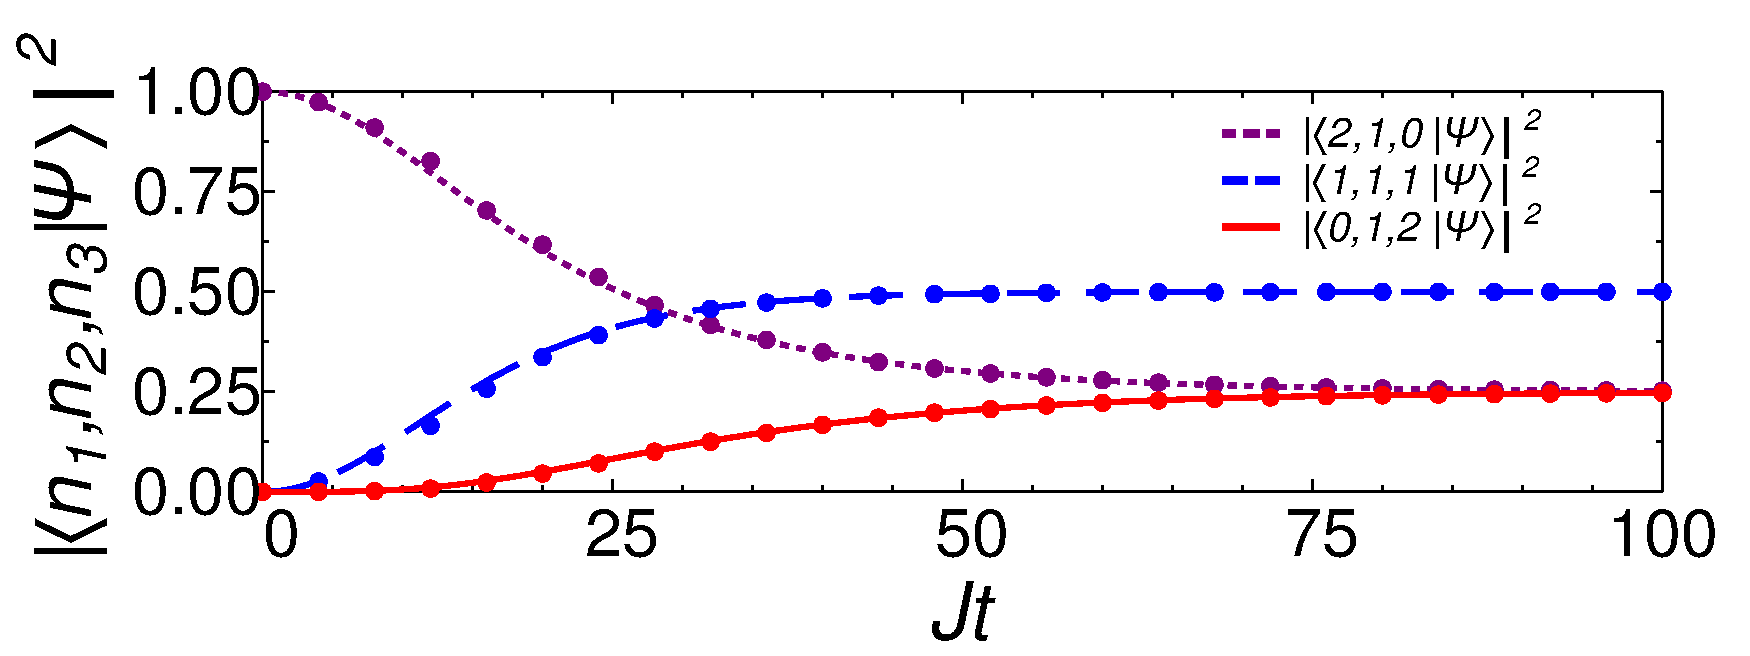
\includegraphics[width=\linewidth]{comp}
	\caption[Fock State Populations in a Zeno
        Subspace]{Populations of the Fock states in the Zeno subspace
          for $\gamma/J = 100$ and initial state $| 2,1,0 \rangle$. It
          is clear that quantum Zeno dynamics occurs via Raman-like
          processes even though none of these states are connected in
          $\hat{H}_0$. The dynamics occurs via virtual intermediate
          states outside the Zeno subspace. The system also tends to a
          steady state which minimises tunnelling effectively
          suppressing fluctuations. The lines are solutions to the
          non-Hermitian Hamiltonian, and the dots are points from a
          stochastic trajectory calculation.\label{fig:comp}}
\end{figure}

\subsection{Steady State of non-Hermitian Dynamics}

A distinctive difference between Bose-Hubbard model ground states and
the final steady state,
$| \Psi \rangle = [|2,1,0 \rangle - \sqrt{2} |1,1,1\rangle +
|0,1,2\rangle]/2$, is that its components are not in phase. Squeezing
due to measurement naturally competes with inter-site tunnelling which
tends to spread the atoms. However, from Eq. \eqref{eq:nHH2} we see
the final state will always be the eigenvector with the smallest
fluctuations as it will have an eigenvalue with the largest imaginary
component. This naturally corresponds to the state where tunnelling
between Zeno subspaces (here between every site) is minimised by
destructive matter-wave interference, i.e.~the tunnelling dark state
defined by $\hat{T} |\Psi \rangle = 0$, where
$\hat{T} = \sum_{\langle i, j \rangle} \bd_i b_j$. This is simply the
physical interpretation of the steady states we predicted for
Eq. \eqref{eq:master}. Crucially, this state can only be reached if
the dynamics aren't fully suppressed by measurement and thus,
counter-intuitively, the atomic dynamics cooperate with measurement to
suppress itself by destructive interference. Therefore, this effect is
beyond the scope of traditional quantum Zeno dynamics and presents a
new perspective on the competition between a system's short-range
dynamics and global measurement backaction.

We now consider a one-dimensional lattice with $M$ sites so we extend
the measurement to $\hat{D} = \N_\text{even}$ where every even site is
illuminated.  The wavefunction in a Zeno subspace must be an
eigenstate of $\c$ and we combine this with the requirement for it to
be in the dark state of the tunnelling operator (eigenstate of $\H_0$
for $U = 0$) to derive the steady state. These two conditions in
momentum space are
\begin{equation}
  \hat{T} | \Psi \rangle = \sum_{\text{RBZ}} \left[ \bd_k b_k -
    \bd_{q} b_{q} \right] \cos(ka) |\Psi \rangle = 0, \nonumber
\end{equation}
\begin{equation}
  \Delta \N |\Psi \rangle = \sum_{\text{RBZ}} \left[ \bd_k b_{-q} +
    \bd_{-q} b_k \right] | \Psi \rangle= \Delta N |\Psi \rangle, \nonumber
\end{equation}
where $b_k = \frac{1}{\sqrt{M}} \sum_j e^{i k j a} b_j$,
$\Delta \hat{N} = \hat{D} - N/2$, $q = \pi/a - k$, $a$ is the lattice
spacing, $N$ the total atom number, and we perform summations over the
reduced Brillouin zone (RBZ), $-\pi/2a < k \le \pi/2a$, as the
symmetries of the system are clearer this way. Now we define
\begin{equation}
\hat{\alpha}_k^\dagger = \bd_k \bd_q - \bd_{-k} \bd_{-q},
\end{equation}
\begin{equation}
\hat{\beta}_\varphi^\dagger = \bd_{\pi/2a} + \varphi \bd_{-\pi/2a},
\end{equation}
where $\varphi = \Delta N / | \Delta N |$, which create the smallest
possible states that satisfy the two equations for $\Delta N = 0$ and
$\Delta N \ne 0$ respectively. Therefore, by noting that
\begin{align}
  \left[ \hat{T}, \hat{\alpha}_k^\dagger \right] & = 0, \\
  \left[ \hat{T}, \hat{\beta}_\varphi^\dagger \right] & = 0, \\
  \left[ \Delta \N, \hat{\alpha}_k^\dagger \right] & = 0, \\
  \left[ \Delta \N, \hat{\beta}_\varphi^\dagger \right] & = \varphi
  \hat{\beta}_\varphi^\dagger,
\end{align}
we can now write the equation for the $N$-particle steady state
\begin{equation}
  \label{eq:ss}
  | \Psi \rangle \propto \left[ \prod_{i=1}^{(N - |\Delta N|)/2}
    \left( \sum_{k = 0}^{\pi/2a} \phi_{i,k} \hat{\alpha}_k^\dagger
    \right) \right] \left( \hat{\beta}_\varphi^\dagger \right)^{|
    \Delta N |} | 0 \rangle, \nonumber
\end{equation}
where $\phi_{i,k}$ are coefficients that depend on the trajectory
taken to reach this state and $|0 \rangle$ is the vacuum state defined
by $b_k |0 \rangle = 0$. Since this a dark state (an eigenstate of
$\H_0$) of the atomic dynamics, this state will remain stationary even
with measurement switched-off. Interestingly, this state is very
different from the ground states of the Bose-Hubbard Hamiltonian, it
is even orthogonal to the superfluid state, and thus it cannot be
obtained by cooling or projecting from an initial ground state. The
combination of tunnelling with measurement is necessary.

\begin{figure}[hbtp!]
	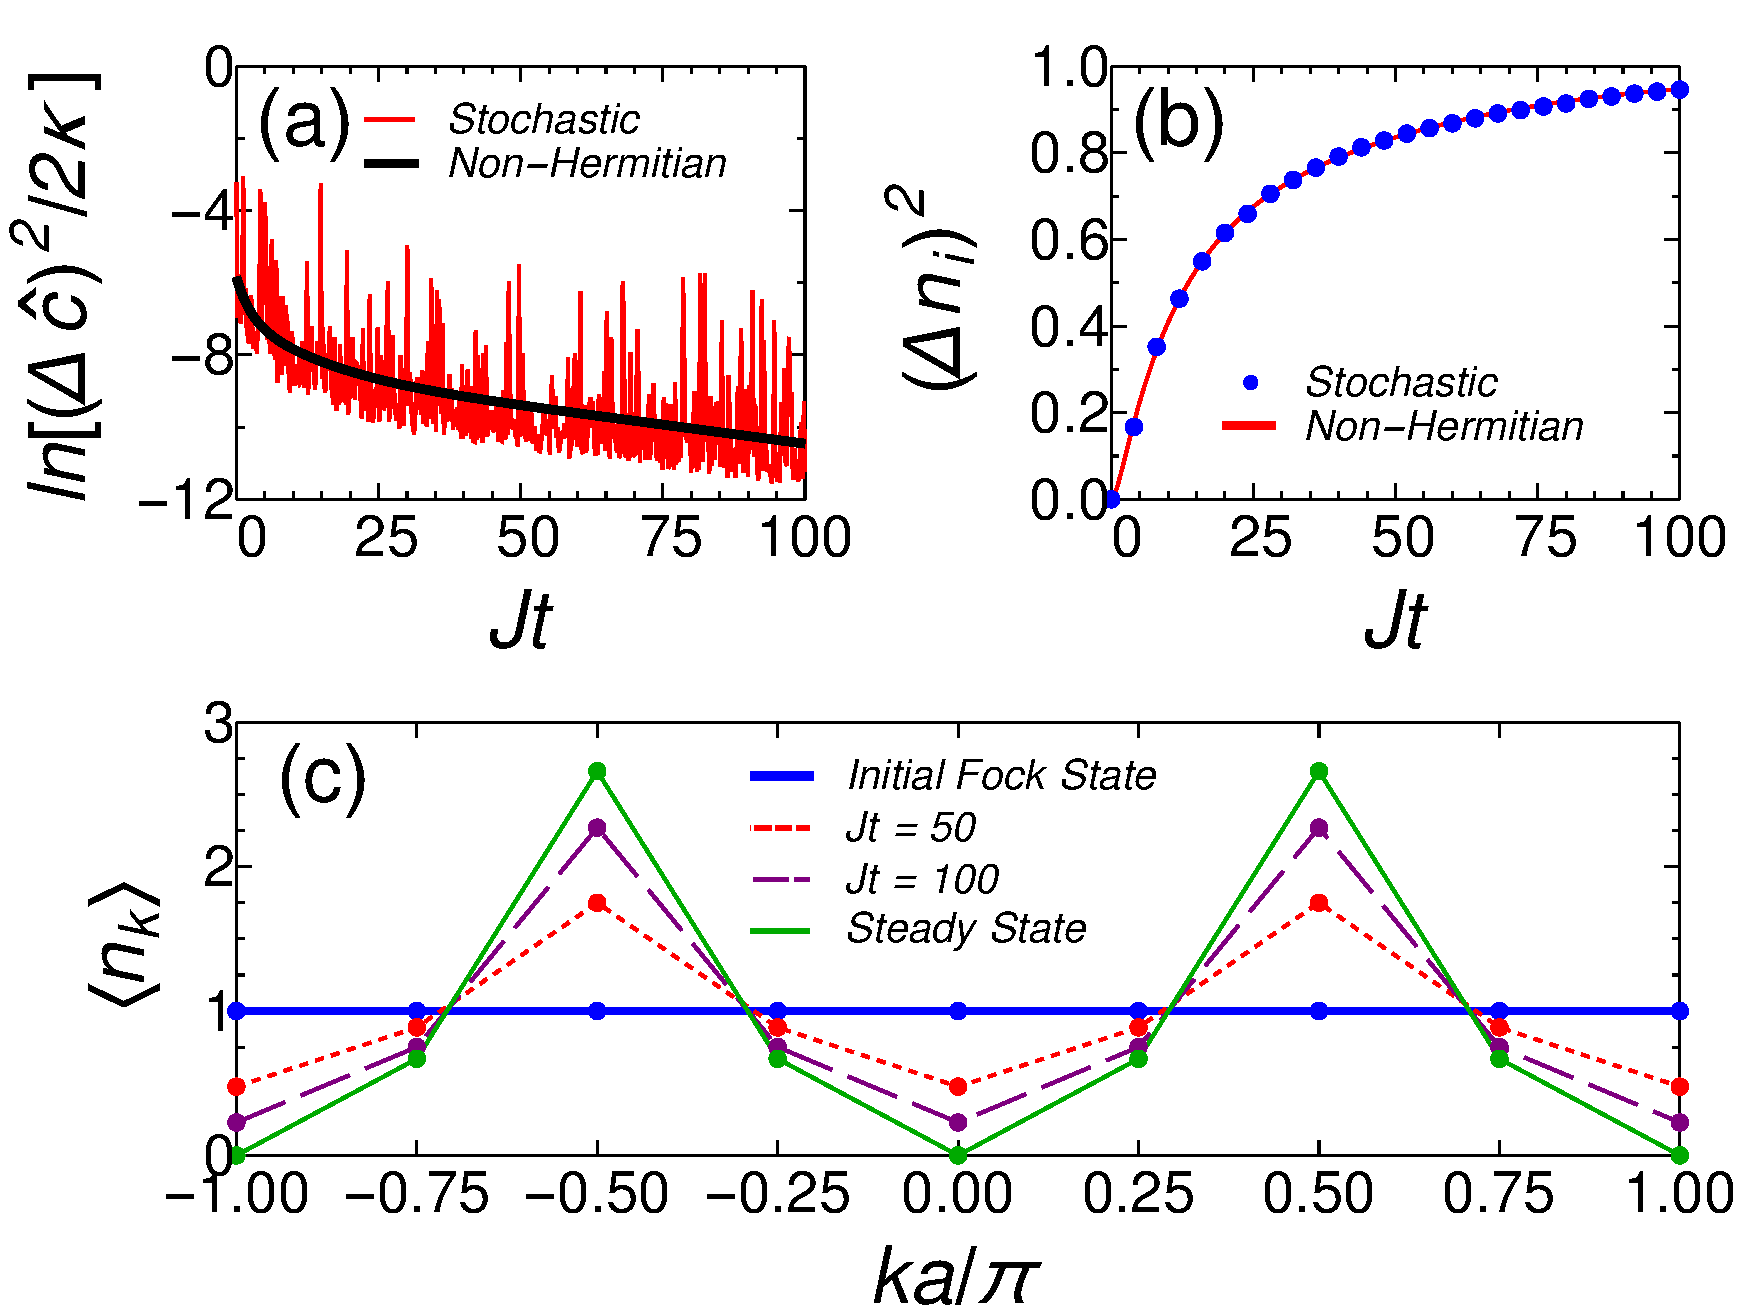
\includegraphics[width=\linewidth]{figure3}
	\caption[Non-Hermitian Steady State]{A trajectory simulation
          for eight atoms in eight sites, initially in
          $|1,1,1,1,1,1,1,1 \rangle$, with periodic boundary
          conditions and $\gamma/J = 100$. (a), The fluctuations in
          $\c$ where the stochastic nature of the process is clearly
          visible on a single trajectory level. However, the general
          trend is captured by the non-Hermitian Hamiltonian. (b), The
          local density variance. Whilst the fluctuations in the
          global measurement operator decrease, the fluctuations in
          local density increase due to tunnelling via states outside
          the Zeno subspace. (c), The momentum distribution. The
          initial Fock state has a flat distribution which with time
          approaches the steady state distribution of two identical
          and symmetric distributions centred at $k = \pi/2a$ and
          $k = -\pi/2a$.\label{fig:steady}}
\end{figure}

In order to prepare the steady state one has to run the experiment and
wait until the photocount rate remains constant for a sufficiently
long time. Such a trajectory is illustrated in Fig. \ref{fig:steady}
and compared to a deterministic trajectory calculated using the
non-Hermitian Hamiltonian. It is easy to see from
Fig. \ref{fig:steady}(a) how the stochastic fluctuations around the
mean value of the observable have no effect on the general behaviour
of the system in the strong measurement regime. By discarding these
fluctuations we no longer describe a pure state, but we showed how
this only leads to a negligible error. Fig. \ref{fig:steady}(b) shows
the local density variance in the lattice. Not only does it grow
showing evidence of tunnelling between illuminated and non-illuminated
sites, but it grows to significant values. This is in contrast to
conventional quantum Zeno dynamics where no tunnelling would be
allowed at all. Finally, Fig. \ref{fig:steady}(c) shows the momentum
distribution of the trajectory. We can clearly see that it deviates
significantly from the initial flat distribution of the Fock
state. Furthermore, the steady state does not have any atoms in the
$k=0$ state and thus is orthogonal to the superfluid state as
discussed.

To obtain a state with a specific value of $\Delta N$ postselection
may be necessary, but otherwise it is not needed.  The process can be
optimised by feedback control since the state is monitored at all
times \cite{ivanov2014}. Furthermore, the form of the measurement
operator is very flexible and it can easily be engineered by the
geometry of the optical setup \cite{elliott2015, mazzucchi2016} which
can be used to design a state with desired properties.

\section{Conclusions}

In this chapter we have demonstrated that global quantum measurement
backaction can efficiently compete with standard local processes in
many-body systems. This introduces a completely new energy and time
scale into quantum many-body research. This is made possbile by the
ability to structure the spatial profile of the measurement on a
microscopic scale comparable to the lattice period without the need
for single site addressing. The extreme flexibility of the setup
considered allowed us to effectively tailor long-range entanglement
and correlations present in the system. We showed that the competition
between the global backaction and usual atomic dynamics leads to the
production of spatially multimode macroscopic superpositions which
exhibit large-scale oscillatory dynamics which could be used for
quantum information and metrology. We subsequently demonstrated that
when on-site atomic interactions are introduced the dynamics become
much more complicated with different regimes of behaviour where
measurement and interactions can either compete or cooperate. In the
strong measurement regime we showed that conventional quantum Zeno
dynamics can be realised, but more interestingly, by considering a
strong, but not projective, limit of measurement we observe a new type
of nonlocal dynamics. It turns out that a global measurement scheme
leads to correlations between spatially separated tunnelling events
which conserve the Zeno subspace via Raman-like processes which would
be forbidden in the canonical fully projective limit. We subsequently
presented a rigorous analysis of the underlying process of this new
type of quantum Zeno dynamics in which we showed that in this limit
quantum trajectories can be described by a deterministic non-Hermitian
Hamiltonian. In contrast to previous works, it is independent of the
underlying system and there is no need to postselect a particular
exotic trajectory \cite{lee2014prx, lee2014prl}. Finally, we have
shown that the system will always tend towards the eigenstate of the
Hamiltonian with the best squeezing of the observable and the atomic
dynamics, which normally tend to spread the distribution, cooperates
with measurement to produce a state in which tunnelling is suppressed
by destructive matter-wave interference. A dark state of the
tunnelling operator will have zero fluctuations and we provided an
expression for the steady state which is significantly different from
the ground state of the Hamiltonian. This is in contrast to previous
works on dissipative state preparation where the steady state had to
be a dark state of the measurement operator \cite{diehl2008}.

Such globally paired tunnelling due to a fundamentally new phenomenon,
global quantum measurement backaction, can enrich the physics of
long-range correlated systems beyond relatively short-range
interactions expected from standard dipole-dipole interactions
\cite{sowinski2012, omjyoti2015}. These nonlocal high-order processes
entangle regions of the optical lattice that are disconnected by the
measurement. Using different detection schemes, we showed how to
tailor density-density correlations between distant lattice
sites. Quantum optical engineering of nonlocal coupling to
environment, combined with quantum measurement, can allow the design
of nontrivial system-bath interactions, enabling new links to quantum
simulations~\cite{stannigel2013} and thermodynamics~\cite{erez2008}
and extend these directions to the field of non-Hermitian quantum
mechanics, where quantum optical setups are particularly
promising~\cite{lee2014prl}. Importantly, both systems and baths,
designed by our method, can be strongly correlated systems with
internal long-range entanglement.
